\documentclass[11pt,a4paper]{article}

% ---------------------------------------------------------------------------
% Rest--rhythm bistability and single-rate switching in the sequential
% distributive three-site phosphorylation cycle
%
% Author metadata: set the three macros below before submission.
% They are deliberately left blank in this version.
% ---------------------------------------------------------------------------
\newcommand{\PaperAuthor}{}
\newcommand{\PaperAffiliation}{}
\newcommand{\PaperDate}{20 September 2026}

\usepackage[T1]{fontenc}
\usepackage[utf8]{inputenc}
\usepackage{lmodern}
\usepackage{microtype}
\usepackage[a4paper,margin=1.05in]{geometry}
\usepackage{amsmath,amssymb,amsthm,mathtools}
\usepackage{booktabs}
\usepackage{array}
\usepackage{enumitem}
\usepackage{xcolor}
\usepackage{graphicx}
\usepackage{tikz}
\usetikzlibrary{arrows.meta,positioning,calc}
\usepackage[numbers,sort&compress]{natbib}
\usepackage[colorlinks=true,linkcolor=blue!55!black,citecolor=blue!55!black,urlcolor=blue!55!black]{hyperref}
\hypersetup{pdftitle={Rest-rhythm bistability and single-rate switching in the sequential distributive three-site phosphorylation cycle},
  pdfkeywords={multisite phosphorylation, futile cycle, generalized Hopf bifurcation, Bautin bifurcation, hard excitation, bistability, limit cycle, nonlinear control, controllability, computer-assisted proof, interval arithmetic}}

\setlist{itemsep=2pt,topsep=3pt}
\setlength{\emergencystretch}{1.5em}
\graphicspath{{figures/}}

\theoremstyle{plain}
\newtheorem{theorem}{Theorem}[section]
\newtheorem{proposition}[theorem]{Proposition}
\newtheorem{lemma}[theorem]{Lemma}
\newtheorem{corollary}[theorem]{Corollary}
\theoremstyle{definition}
\newtheorem{definition}[theorem]{Definition}
\newtheorem{question}[theorem]{Question}
\theoremstyle{remark}
\newtheorem{remark}[theorem]{Remark}

\newcommand{\R}{\mathbb R}
\newcommand{\C}{\mathbb C}
\newcommand{\Z}{\mathbb Z}
\newcommand{\ii}{\mathrm i}
\newcommand{\T}{\mathsf T}
\newcommand{\cN}{\mathcal N}
\newcommand{\cL}{\mathcal L}
\newcommand{\cE}{\mathcal E}
\newcommand{\cW}{\mathcal W}
\newcommand{\ET}{E_{\mathrm T}}
\newcommand{\FT}{F_{\mathrm T}}
\newcommand{\ST}{S_{\mathrm T}}
\newcommand{\GH}{\mathrm{GH}}
\newcommand{\norm}[1]{\lVert#1\rVert}
\newcommand{\abs}[1]{\lvert#1\rvert}
\DeclareMathOperator{\Ree}{Re}
\DeclareMathOperator{\Imm}{Im}
\DeclareMathOperator{\rank}{rank}
\newcommand{\evC}{\textsf{C}}
\newcommand{\evI}{\textsf{I}}
\newcommand{\evK}{\textsf{K}}
\newcommand{\evN}{\textsf{N}}

\title{Rest--rhythm bistability and single-rate switching\\ in the sequential distributive three-site\\ phosphorylation cycle}
\author{\PaperAuthor\\[2pt]\small\PaperAffiliation}
\date{\PaperDate}

\begin{document}
\maketitle

\begin{abstract}
The sequential, fully distributive $n$-site phosphorylation cycle with one kinase and one phosphatase contains no feedback reaction, yet for $n=3$ it was recently shown to possess attracting periodic orbits. We prove that the same mass-action network can do more: for one fixed list of eighteen positive rate constants and one fixed triple of conserved totals it has a linearly stable positive steady state (\emph{rest}) and, simultaneously, an orbitally asymptotically stable positive periodic orbit (\emph{rhythm}). The proof locates a generalized Hopf (Bautin) point in an explicit rational two-parameter family of rate constants: a directed-interval Newton--Kantorovich certificate gives a unique parameter point with a simple imaginary pair, seven stable complementary eigenvalues, vanishing first Lyapunov coefficient, real quintic normal-form coefficient in $(-0.044427531,-0.044427474)$ and a regular two-parameter unfolding. The unfolding theorem then yields a wedge of parameters with a sink, an unstable cycle and an attracting cycle, and hyperbolicity makes coexistence an open property of all eighteen rates and three totals. A separate, exactly specified witness makes the statement quantitative: two independent computer-assisted proofs, a Fourier contraction with a validated return map and a multiple-shooting Newton--Kantorovich argument, establish a positive attracting periodic orbit with period in $(28.69124274158,28.69124274167)$ whose peak-to-peak variation of the fully phosphorylated pool exceeds $2.3456$, with leading Floquet multiplier enclosed in $[0.888,0.972]$, and its equilibrium is a certified sink; in the one-parameter family through this witness the equilibrium loses stability in a certified \emph{subcritical} Hopf bifurcation. We then ask how little actuation is needed to switch between the two behaviours. At the generalized Hopf point the linearization is controllable from a \emph{single} rate constant, and this is true for every one of the eighteen rate constants (interval Kalman rank certificates). A parameter-uniform endpoint argument converts this into a theorem: for every prescribed duration and every bound $0<\eta<1$ on the relative modulation there are coexisting baselines, arbitrarily close to the generalized Hopf point, at which smooth modulation of one rate constant alone, with all other rates and all totals untouched, steers rest exactly onto the cycle and any chosen point of the cycle exactly to rest, with open sets of tolerated preparation and actuation errors. At the finite witness, where no switching theorem is claimed, a $\pm10\%$ resonant modulation of one phosphatase association constant over three periods toggles both ways in simulation. We state precisely which assertions are conventional mathematics, which are interval-certified, which are numerical, and what remains open.
\end{abstract}

\tableofcontents

\section{Introduction}\label{sec:intro}

\subsection{The model and the question}
Reversible phosphorylation of a protein at several sites is one of the most common regulatory motifs of the cell \cite{Cohen00}. In the \emph{sequential distributive} mechanism a kinase $E$ adds phosphate groups one at a time and in a fixed order, releasing the substrate after each catalytic event, and a phosphatase $F$ removes them in the reverse order in the same manner. Writing $S_i$ for the substrate with $i$ phosphorylated sites, $C_i=S_{i-1}E$ for the kinase complexes and $D_i=S_iF$ for the phosphatase complexes, the three-site network $\cN_3$ is
\begin{equation}\label{eq:network}
 S_{i-1}+E \underset{b_i}{\overset{a_i}{\rightleftharpoons}} C_i
 \overset{c_i}{\longrightarrow}S_i+E,\qquad
 S_i+F \underset{\beta_i}{\overset{\alpha_i}{\rightleftharpoons}}D_i
 \overset{\gamma_i}{\longrightarrow}S_{i-1}+F,
 \qquad i=1,2,3,
\end{equation}
with mass-action kinetics and eighteen positive rate constants (Figure~\ref{fig:network}). There are twelve species, ordered throughout as
\[
 x=(S_0,S_1,S_2,S_3,E,F,C_1,C_2,C_3,D_1,D_2,D_3),
\]
and three conserved totals
\begin{equation}\label{eq:totals}
 \ET=E+\sum_{i=1}^3 C_i,\qquad \FT=F+\sum_{i=1}^3 D_i,\qquad
 \ST=\sum_{j=0}^3S_j+\sum_{i=1}^3(C_i+D_i),
\end{equation}
so that the dynamics takes place on nine-dimensional compatibility classes. Every statement about stability or attraction in this paper is relative to a fixed compatibility class. No allosteric, transcriptional or product-inhibition feedback is present in \eqref{eq:network}; the only coupling between the sites is that all six complexes draw on the same two enzyme pools.

The steady states of the $n$-site network $\cN_n$ are well understood: there is a unique globally attracting equilibrium for $n=1$ \cite{AngeliSontag08}, and multistationarity for $n\ge2$ \cite{Markevich04,WangSontag08a,ConradiMincheva14,HellRendall15}, with up to $2n-1$ equilibria \cite{WangSontag08a,Flockerzi14} and a number of stable equilibria growing with $n$ \cite{ThomsonGunawardena09,FeliuRendallWiuf20}. Oscillations proved far more elusive \cite{ConradiShiu18,ConradiFeliuMincheva20,FeliuKaihnsa26}. Vassena \cite{Vassena26} showed that the mass-action dual cycle $\cN_2$ has no nonzero purely imaginary eigenvalue at any positive equilibrium, hence no Hopf bifurcation, and left $n\ge3$ open; this excludes Hopf bifurcation for $n=2$ but, by itself, neither global convergence nor every conceivable periodic orbit. The companion paper \cite{CompanionOscillations} settled the case $n\ge3$: $\cN_3$ has a supercritical Hopf bifurcation with certified first Lyapunov coefficient $l_1=-0.0891594\ldots$ (``witness~$\mathsf A$''), hence orbitally asymptotically stable positive periodic orbits, and also a subcritical one with $l_1>0$ (``witness~$\mathsf H$''); both witnesses are instances of the equilibrium--flux parametrization \eqref{eq:rates} below, and a site-addition argument carries the result to every $n\ge3$. Oscillations had earlier been found only in \emph{modified} multisite systems, for example with a mixed processive/distributive mechanism \cite{SuwanmajoKrishnan15,ConradiMinchevaShiu19} or a random order of sites \cite{Jolley12}; those are different reaction architectures.

Two Hopf points of opposite criticality in one connected family suggest a codimension-two organizing centre between them: a \emph{generalized Hopf} (Bautin) point \cite{Bautin52,Takens73,GolubitskyLangford81,Kuznetsov23}, at which the first Lyapunov coefficient vanishes. If the second Lyapunov coefficient is negative there, the unfolding contains a parameter region with \emph{three} nested invariant objects: a stable equilibrium, an unstable periodic orbit around it, and a stable periodic orbit around both. This is the classical scenario of \emph{hard excitation} \cite{Goldbeter96}: a system that is silent when left alone, oscillates indefinitely after a sufficiently large perturbation, and can be silenced again by a suitably timed stimulus, as in the annihilation experiments on the squid axon \cite{GuttmanLewisRinzel80,Winfree01}. Small planar mass-action networks are known to admit Bautin bifurcations \cite{BanajiBorosHofbauer24}. The questions addressed here are whether the literal phosphorylation network \eqref{eq:network} realizes this scenario, whether that can be proved rather than simulated, and how little external actuation suffices to switch it.

We use the term \emph{rest--rhythm bistability} for the coexistence of a stable equilibrium with a stable periodic orbit at the same parameters in the same compatibility class. (``Birhythmicity'' conventionally means two coexisting stable \emph{oscillations} and is not what is meant.)

\begin{figure}[t]
\centering
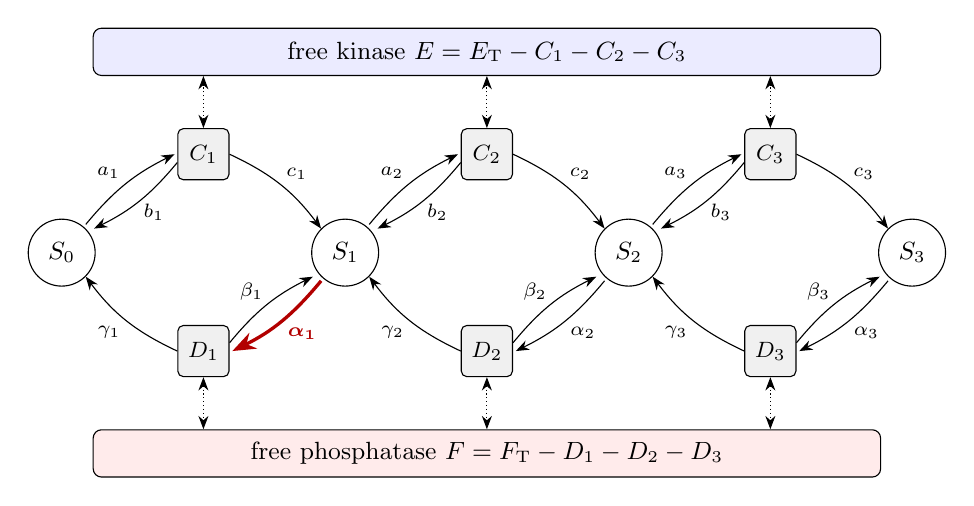
\begin{tikzpicture}[>=Stealth,node distance=20mm,
  sp/.style={circle,draw,minimum size=8.5mm,inner sep=0pt,font=\small},
  cx/.style={rectangle,rounded corners=2pt,draw,minimum size=6.5mm,inner sep=1.5pt,font=\footnotesize,fill=black!6}]
\node[sp] (S0) at (0,0) {$S_0$};
\node[sp] (S1) at (3.6,0) {$S_1$};
\node[sp] (S2) at (7.2,0) {$S_2$};
\node[sp] (S3) at (10.8,0) {$S_3$};
\foreach \i/\a/\b in {1/S0/S1,2/S1/S2,3/S2/S3}{
  \node[cx] (C\i) at ($(\a)!0.5!(\b)+(0,1.25)$) {$C_\i$};
  \node[cx] (D\i) at ($(\a)!0.5!(\b)+(0,-1.25)$) {$D_\i$};
  \draw[->] ([yshift=1.5pt]\a.north east) to[bend left=12] node[above left=-2pt,font=\scriptsize]{$a_\i$} ([xshift=-1pt]C\i.west);
  \draw[->] ([yshift=-3pt]C\i.west) to[bend left=12] node[below right=-3pt,font=\scriptsize]{$b_\i$} ([xshift=3pt]\a.north east);
  \draw[->] (C\i.east) to[bend left=14] node[above right=-2pt,font=\scriptsize]{$c_\i$} (\b.north west);
  \draw[->] ([yshift=3pt]D\i.east) to[bend left=12] node[above left=-3pt,font=\scriptsize]{$\beta_\i$} ([xshift=-3pt]\b.south west);
  \draw[->] (D\i.west) to[bend left=14] node[below left=-2pt,font=\scriptsize]{$\gamma_\i$} (\a.south east);
}
\foreach \i/\b in {2/S2,3/S3}{
  \draw[->] ([yshift=-1.5pt]\b.south west) to[bend left=12] node[below right=-2pt,font=\scriptsize]{$\alpha_\i$} ([xshift=1pt]D\i.east);}
\draw[->,very thick,red!70!black] ([yshift=-1.5pt]S1.south west) to[bend left=12] node[below right=-2pt,font=\scriptsize]{$\boldsymbol{\alpha_1}$} ([xshift=1pt]D1.east);
\node[draw,rounded corners=3pt,fill=blue!8,minimum width=100mm,minimum height=6mm,font=\small] (E) at (5.4,2.55) {free kinase $E=\ET-C_1-C_2-C_3$};
\node[draw,rounded corners=3pt,fill=red!8,minimum width=100mm,minimum height=6mm,font=\small] (F) at (5.4,-2.55) {free phosphatase $F=\FT-D_1-D_2-D_3$};
\foreach \i in {1,2,3}{\draw[densely dotted,<->] (C\i.north) -- (C\i.north|-E.south);
                       \draw[densely dotted,<->] (D\i.south) -- (D\i.south|-F.north);}
\end{tikzpicture}
\caption{The three-site sequential distributive cycle $\cN_3$. Each complex is formed reversibly and resolved irreversibly; all six complexes draw on the two shared free-enzyme pools (dotted), and this is the only interaction between sites. The thick arrow marks the single rate constant that is modulated, $\alpha_1\mapsto\alpha_1(1+u(t))$, in the switching theorem and in Figure~\ref{fig:switch}; Proposition~\ref{prop:rank} shows that any of the other seventeen would serve equally.}
\label{fig:network}
\end{figure}

\subsection{Results}

\begin{theorem}[Rest--rhythm bistability]\label{thm:coexist}
There are eighteen positive mass-action rate constants and positive totals $(\ET,\FT,\ST)$ such that the corresponding compatibility class of \eqref{eq:network} contains a positive equilibrium which is a hyperbolic sink and, disjoint from it, a positive nonconstant periodic orbit which is hyperbolic and orbitally asymptotically stable. The set of parameters $(a_i,b_i,c_i,\alpha_i,\beta_i,\gamma_i,\ET,\FT,\ST)\in\R^{21}_{>0}$ with this property has nonempty interior. Such parameters exist in every neighbourhood of the generalized Hopf point of Theorem~\ref{thm:GH}, and there the class contains in addition a hyperbolic periodic orbit with exactly one unstable Floquet multiplier, lying between the sink and the attracting orbit on a two-dimensional invariant manifold.
\end{theorem}

\begin{theorem}[An explicit witness]\label{thm:finite}
Let the rate constants and totals be those reconstructed by \eqref{eq:rates} from the exact dyadic data of Table~\ref{tab:dyadic} $($rounded values in Table~\ref{tab:rates}; $(\ET,\FT,\ST)\approx(4.5333,21.6998,40.3944))$. Then, in the corresponding class,
\begin{enumerate}[label=\textup{(\roman*)},leftmargin=*]
\item the positive equilibrium $x^*$ of Table~\ref{tab:dyadic} is a hyperbolic sink;
\item there is a periodic orbit $\Gamma$ with minimal period $T\in(28.69124274158,\,28.69124274167)$, along which every species concentration is bounded below by a positive constant, and along which the readout $S_3+D_3$ has peak-to-peak variation greater than $2.34560$;
\item all eight nontrivial Floquet multipliers of $\Gamma$ lie in the open unit disc, so $\Gamma$ is hyperbolic and orbitally asymptotically stable; one of them is real and lies in $[0.8881,0.9716]$, one is real and lies in $[0.5219,0.6378]$, and the other six have modulus below $1.7\cdot10^{-3}$;
\item in the one-parameter family obtained by varying the reverse ratio $r$ in \eqref{eq:rates}, the equilibrium $x^*$ undergoes a Hopf bifurcation at $r_{\mathrm H}=1.34467152419\ldots$ with first Lyapunov coefficient $l_1=+0.0472061743\ldots>0$ $($subcritical$)$; $x^*$ is a sink for $r>r_{\mathrm H}$, and the witness has $r=1.35201370\ldots>r_{\mathrm H}$.
\end{enumerate}
\end{theorem}

Items (ii) and (iii) are proved twice, by two computer-assisted arguments that share neither method nor code (Propositions~\ref{prop:fourier} and \ref{prop:shooting}); the enclosures of the individual multipliers come from the second. Numerically the witness also has the unstable cycle predicted by the local theory (period $26.50998$, readout range $1.0276$, unstable multiplier $1.01604$), and the attracting and unstable cycles merge in a fold at $r\approx1.35628$ (Figures~\ref{fig:witness} and \ref{fig:branch}); these numerical statements are not part of Theorem~\ref{thm:finite}.

For the switching theorem, fix one of the eighteen rate constants, call it $k$, and replace it by $k\,(1+u(t))$, where $u$ is a scalar function of time. Nothing else is altered: the other seventeen rate constants are fixed, the totals are conserved because the stoichiometry is unchanged, and outside the support of $u$ the system is the autonomous baseline.

\begin{theorem}[Single-rate switching]\label{thm:switch}
Let $k$ be any one of the eighteen rate constants. Fix a duration $\tau>0$ and a bound $0<\eta<1$. In every neighbourhood of the generalized Hopf point of Theorem~\ref{thm:GH} there are parameters at which \eqref{eq:network} has a sink $x^*$ and an attracting periodic orbit $\Gamma$ as in Theorem~\ref{thm:coexist}, and for which the following holds.
\begin{enumerate}[label=\textup{(\roman*)},leftmargin=*]
\item \emph{ON.} For every $d\in\Gamma$ there is $u\in C_c^\infty((0,\tau))$ with $\norm u_\infty<\eta$ such that the solution of \eqref{eq:network} with $k$ replaced by $k(1+u(t))$ and initial state $x^*$ is at $d$ at time $\tau$.
\item \emph{OFF.} For every $d\in\Gamma$ there is $u_d\in C_c^\infty((0,\tau))$ with $\norm{u_d}_\infty<\eta$ such that the solution with $k$ replaced by $k(1+u_d(t))$ and initial state $d$ is at $x^*$ at time $\tau$. The waveform $u_d$ depends smoothly on $d$.
\item \emph{Positivity.} Along these trajectories all concentrations remain positive, and $k(1+u(t))>0$.
\item \emph{Robustness.} There is $\delta>0$ such that every initial state within $\delta$ of the nominal one in the same class, driven by any measurable input $\tilde u$ with $\norm{\tilde u-u}_\infty<\delta$ on $[0,\tau]$, ends at time $\tau$ in the basin of attraction of the intended attractor. Consequently finitely many OFF waveforms $u_{d_1},\dots,u_{d_m}$ suffice for all phases of $\Gamma$.
\end{enumerate}
For any finite $m$ and any $\epsilon_1,\dots,\epsilon_m>0$ the parameters can in addition be chosen so that $\norm{u^{(j)}}_\infty<\epsilon_j$ for $1\le j\le m$ for all the waveforms above.
\end{theorem}

The quantifiers matter. The theorem asserts that, \emph{given} $\tau$ and $\eta$, suitable coexisting baselines exist near the generalized Hopf point; the admissible neighbourhood shrinks with $\tau$ and $\eta$, and no explicit size is given. It does not assert that the explicit witness of Theorem~\ref{thm:finite} can be switched by one rate constant, although simulation indicates that it can (Section~\ref{sec:demo}). The OFF waveform depends on the phase at which it is applied; a single phase-blind OFF waveform is not claimed (Remark~\ref{rem:phaseblind}). The nine temporal degrees of freedom used in the proof are coefficients of one scalar signal acting on one rate constant, not nine actuators.

\subsection{Method and evidence}\label{sec:evidence}
The proofs combine conventional analysis with validated numerics \cite{Tucker11,vandenBergLessard15}. We label evidence throughout:
\begin{description}[leftmargin=2.2em,labelwidth=1.6em,itemsep=1pt]
\item[\evC] conventional mathematical proof, given or cited in the text;
\item[\evI] a finite computation in directed (outward-rounded) interval arithmetic, or in binary64 arithmetic with explicit forward error bounds, all of whose acceptance conditions are strict inequalities;
\item[\evK] an identity or inequality compiled in Lean~4 with Mathlib \cite{MouraUllrich21,Mathlib20};
\item[\evN] floating-point numerics, used for illustration and cross-checks only.
\end{description}
Theorems~\ref{thm:coexist}--\ref{thm:switch} rest on \evC{} and \evI{} only. The Lean modules check elementary algebraic identities (the equilibrium balance, the input column, a Lyapunov inequality) and play no role in the dynamical arguments; no part of the bifurcation, periodic-orbit or control theory is formalized. Section~\ref{sec:repro} lists every computation, and also records the independent replications carried out for this paper: the normal-form coefficients were recomputed by a second implementation of the centre-manifold recurrence built directly from the reaction list, the sign change of $l_1$ across the generalized Hopf point and the subcritical Hopf point of Theorem~\ref{thm:finite}(iv) were certified with separate rational-interval code, and the existence, period, positivity and stability of the witness orbit were proved a second time by an unrelated method (multiple shooting with interval Taylor integration, Proposition~\ref{prop:shooting}).

\subsection{Organization}
Section~\ref{sec:coords} sets up exact coordinates in which the vector field is quadratic and the equilibrium is prescribed. Section~\ref{sec:GH} certifies the generalized Hopf point and proves Theorem~\ref{thm:coexist}. Section~\ref{sec:finite} treats the finite witness. Section~\ref{sec:control} proves Theorem~\ref{thm:switch} and its corollaries, and illustrates switching at the witness. Section~\ref{sec:physical} gives a dimensional example and discusses readout, noise, fuel and actuation. Section~\ref{sec:repro} states scope, reproducibility and open problems. The appendices contain the exact data, the derivation of the normal-form equations and the checking arguments of the computer-assisted steps.

\section{Exact coordinates}\label{sec:coords}

\subsection{Equilibrium--flux parametrization}
Choose positive concentrations $x^*\in\R^{12}_{>0}$, positive catalytic currents $\phi_1,\phi_2,\phi_3$, and positive reverse ratios $\rho_i,\sigma_i$, and define
\begin{equation}\label{eq:rates}
\begin{aligned}
a_i&=\frac{(1+\rho_i)\phi_i}{S_{i-1}^*E^*},&
b_i&=\frac{\rho_i\phi_i}{C_i^*},&c_i&=\frac{\phi_i}{C_i^*},\\[2pt]
\alpha_i&=\frac{(1+\sigma_i)\phi_i}{S_i^*F^*},&
\beta_i&=\frac{\sigma_i\phi_i}{D_i^*},&\gamma_i&=\frac{\phi_i}{D_i^*}.
\end{aligned}
\end{equation}

\begin{lemma}\label{lem:param}
With the rates \eqref{eq:rates}, $x^*$ is an equilibrium of \eqref{eq:network}. Conversely, every positive equilibrium of \eqref{eq:network} arises in this way from unique $\phi_i,\rho_i,\sigma_i>0$, namely $\phi_i=c_iC_i^*$, $\rho_i=b_i/c_i$ and $\sigma_i=\beta_i/\gamma_i$.
\end{lemma}
\begin{proof}
At $x^*$ the three fluxes of the kinase arm $i$ are $(1+\rho_i)\phi_i$, $\rho_i\phi_i$ and $\phi_i$, so $\dot C_i=(1+\rho_i)\phi_i-\rho_i\phi_i-\phi_i=0$; likewise $\dot D_i=0$. Hence $\dot E=-\sum\dot C_i=0$ and $\dot F=0$. The net binding flux into each complex equals its catalytic flux, so $S_j$ gains $\phi_j$ from the catalytic step of $C_j$ and $\phi_{j+1}$ from that of $D_{j+1}$, and loses $\phi_{j+1}$ by net binding into $C_{j+1}$ and $\phi_j$ by net binding into $D_j$ (with $\phi_0=\phi_4=0$); these cancel. For the converse, $\dot C_i=\dot D_i=0$ determine the association fluxes from the other two, and summing the equations for $S_3,S_2,S_1$ successively gives $c_iC_i^*=\gamma_iD_i^*$.
\end{proof}

The parametrization produces positive sources with a prescribed equilibrium. It does not by itself produce multistability: equilibria reconstructed with \emph{different} rate lists say nothing about coexistence. Every sink/cycle pair below belongs to one rate list and one class.

\subsection{The pool/complex chart}
For $i=1,2,3$ let
\begin{equation}\label{eq:pools}
U_i=\sum_{j=i}^{3}S_j+\sum_{j=i+1}^{3}C_j+\sum_{j=i}^{3}D_j
\end{equation}
be the total concentration of substrate carrying at least $i$ phosphate groups, free or bound ($C_j$ carries $j-1$ groups and $D_j$ carries $j$). Binding and unbinding do not change the phosphorylation level, so
\begin{equation}\label{eq:pooldot}
\dot U_i=c_iC_i-\gamma_iD_i .
\end{equation}
In particular the readout of Theorem~\ref{thm:finite} is a chart coordinate: $S_3+D_3=U_3$.

Given the totals, $(U_1,U_2,U_3,C_1,C_2,C_3,D_1,D_2,D_3)$ are global coordinates on the class. We use displacements from a reference point $x^*$ of the class,
\[
y=(\pi_1,\pi_2,\pi_3,\;\xi_1,\xi_2,\xi_3,\;\zeta_1,\zeta_2,\zeta_3),\qquad
\pi_i=U_i-U_i^*,\quad \xi_i=C_i-C_i^*,\quad \zeta_i=D_i-D_i^*,
\]
and write $e_{\pi_i},e_{C_i},e_{D_i}$ for the corresponding unit vectors of $\R^9$. The inverse is the affine map $x=x^*+Py$ with
\begin{equation}\label{eq:lift}
Py=\bigl(-\pi_1-\xi_1,\;\pi_1-\pi_2-\xi_2-\zeta_1,\;\pi_2-\pi_3-\xi_3-\zeta_2,\;\pi_3-\zeta_3,\;
-\textstyle\sum_i\xi_i,\;-\sum_i\zeta_i,\;\xi,\;\zeta\bigr).
\end{equation}
The matrix $P\in\Z^{12\times9}$ has rank nine, its image is the stoichiometric subspace (it annihilates the three totals), and the pool/complex projection $R\in\Z^{9\times12}$ defined by \eqref{eq:pools} satisfies $RP=I_9$.

\begin{lemma}\label{lem:quadratic}
Let $x^*$ be an equilibrium. In the chart, the restriction of \eqref{eq:network} to the class of $x^*$ is exactly
\begin{equation}\label{eq:field}
\dot y=f(y)=Jy+\tfrac12B(y,y),
\end{equation}
with a constant matrix $J$ and a constant symmetric bilinear map $B$. The $\pi$-rows of $J$ are $c_ie_{C_i}^\T-\gamma_ie_{D_i}^\T$ and the $\pi$-components of $B$ vanish. For a complex $Z\in\{C_i,D_i\}$ formed from substrate form $S_{l}$ and enzyme $G\in\{E,F\}$ with association constant $\kappa$, dissociation constant $\kappa'$ and catalytic constant $\kappa''$, and with $P_l,P_G$ the corresponding rows of $P$,
\begin{equation}\label{eq:JB}
J_{Z,\cdot}=\kappa\,(G^*P_{l}+S_l^*P_{G})-(\kappa'+\kappa'')\,e_Z^\T,\qquad
B_Z(p,p')=\kappa\,\bigl[(P_lp)(P_Gp')+(P_lp')(P_Gp)\bigr].
\end{equation}
\end{lemma}
\begin{proof}
Equation \eqref{eq:pooldot} is linear, and $\dot Z=\kappa S_lG-(\kappa'+\kappa'')Z$ is a quadratic polynomial in $x=x^*+Py$ whose constant term vanishes because $x^*$ is an equilibrium.
\end{proof}

No Michaelis--Menten or quasi-steady-state reduction is made anywhere: \eqref{eq:field} is the literal mass-action system. Exact quadraticity simplifies derivative computations, but the dynamics on a centre manifold is of course not quadratic; cubic and quintic terms arise through the manifold.

If the totals are varied, the reference point can be moved smoothly (for instance $x^*+\delta_E e_E+\delta_Fe_F+\delta_Se_{S_0}$), so in the chart the vector field depends smoothly on all eighteen rates and three totals on one fixed open subset of $\R^9$.

\subsection{Normal-form conventions}\label{sec:nf}
Suppose $J$ has a simple eigenvalue $\ii\omega$, $\omega>0$, and no other eigenvalues on the imaginary axis besides $-\ii\omega$. Let $Jq=\ii\omega q$ and $\ell^\T J=\ii\omega\,\ell^\T$ with the \emph{bilinear} normalization $\ell^\T q=1$ (no complex conjugation; then $\ell^\T\bar q=0$), and fix $q_{D_3}=1$. There is a parametrization $y=H(z,\bar z)=zq+\bar z\bar q+\sum_{j+k\ge2}h_{jk}z^j\bar z^k/(j!\,k!)$ of a centre manifold on which
\begin{equation}\label{eq:nf}
\dot z=\ii\omega z+G_1z\abs z^2+G_2z\abs z^4+O(\abs z^7),
\end{equation}
with physical time unchanged. The Lyapunov coefficients in the convention of \cite{Kuznetsov23} are $l_1=\Ree G_1/\omega$ and, when $l_1=0$, $l_2=\Ree G_2/\omega$; only the signs of $\Ree G_1$ and $\Ree G_2$ and the nonvanishing of a Jacobian matter below, and these do not depend on the normalization of $q$. With $L_m=m\ii\omega I-J$ the coefficients are given by
\begin{align}
&L_2h_{20}=B(q,q),\qquad L_0h_{11}=B(q,\bar q),\qquad
G_1=\tfrac12\,\ell^\T\bigl[2B(q,h_{11})+B(\bar q,h_{20})\bigr],\label{eq:G1}\\
&L_1h_{21}=2B(q,h_{11})+B(\bar q,h_{20})-2G_1q,\quad \ell^\T h_{21}=0,\qquad L_3h_{30}=3B(q,h_{20}),\notag\\
&L_2h_{31}=3B(q,h_{21})+B(\bar q,h_{30})+3B(h_{11},h_{20})-6G_1h_{20},\notag\\
&L_0h_{22}=2B(q,\bar h_{21})+2B(\bar q,h_{21})+B(h_{20},\bar h_{20})+2B(h_{11},h_{11})-4(G_1+\bar G_1)h_{11},\notag\\
&12\,G_2=\ell^\T\bigl[3B(q,h_{22})+2B(\bar q,h_{31})+B(\bar h_{20},h_{30})+6B(h_{11},h_{21})+3B(\bar h_{21},h_{20})\bigr].\label{eq:G2}
\end{align}
These equations are derived in Appendix~\ref{app:nf}; the term $-4(G_1+\bar G_1)h_{11}=-8(\Ree G_1)h_{11}$ in the equation for $h_{22}$ vanishes at a generalized Hopf point and is kept only so that the formulas extend smoothly to a neighbourhood.

\section{A certified generalized Hopf point}\label{sec:GH}

\subsection{The rational patch}
Let $x_0,v\in\R^{12}$ and $\phi_0,w\in\R^3$ be the exact decimal vectors of Table~\ref{tab:patch}, and for parameters $\mu=(s,r)$ put
\begin{equation}\label{eq:patch}
x^*(s)=x_0+sv,\qquad \phi(s)=\phi_0+sw,\qquad \rho_1=\rho_2=\rho_3=\sigma_2=\sigma_3=\tfrac1{100},\qquad\sigma_1=r,
\end{equation}
on the patch $\abs s\le10^{-6}$, $1.38378\le r\le1.38380$, where all concentrations, currents and rates are positive (\evI). By Lemma~\ref{lem:param}, $x^*(s)$ is an equilibrium for every $\mu$, so in the chart centred at $x^*(s)$ we obtain a smooth two-parameter family $f_\mu(y)=J_\mu y+\frac12B_\mu(y,y)$ with $f_\mu(0)=0$. The point $x_0$ lies on the log-linear path between the witnesses $\mathsf H$ and $\mathsf A$ of \cite{CompanionOscillations}, at the place where numerics indicated the sign change of $l_1$; $v$ and $w$ are the path directions. The reverse ratio $r=\beta_1/\gamma_1$ enters only $\alpha_1$ and $\beta_1$.

\subsection{The zero problem}
Let $A=\ii\omega I-J_\mu$. Solve the first eight rows of $Aq=0$ with $q_{D_3}=1$, solve the first eight rows of $A^\T\ell_0=0$ with last component one, and put $\ell=\ell_0/(\ell_0^\T q)$. Define $h_{20},h_{11},G_1$ by \eqref{eq:G1} with these vectors. All of this is an explicit rational function of $(s,r,\omega)$ wherever the two $8\times8$ minors, $\ell_0^\T q$, $\det J_\mu$ and $\det L_2$ are nonzero. Consider the three real equations
\begin{equation}\label{eq:zero}
\mathcal F(s,r,\omega)=\bigl(\Ree (Aq)_9,\ \Imm (Aq)_9,\ \Ree G_1\bigr)=0 .
\end{equation}
At a zero, $q$ is an eigenvector for $\ii\omega$; then $\det A=0$, the transposed $8\times8$ system has the same nonzero minor, and the last equation of $A^\T\ell_0=0$ holds automatically (Schur complement), so $\ell$ is the normalized left eigenvector and $G_1$ is the true cubic normal-form coefficient.

\begin{theorem}[\evI]\label{thm:GH}
Let $(\bar s,\bar r,\bar\omega)$ be the decimal triple
\[
\bar s=-7.13271936896\ldots\cdot10^{-14},\qquad \bar r=1.38378737705141\ldots,\qquad\bar\omega=0.241811388817579\ldots
\]
given to fifty digits in Appendix~\ref{app:data}. In the box $\{\norm{(s,r,\omega)-(\bar s,\bar r,\bar\omega)}_\infty\le10^{-20}\}$ the system \eqref{eq:zero} has exactly one zero $(s_0,r_0,\omega_0)$, and it lies within $3.084\cdot10^{-30}$ of the centre. At $\mu_0=(s_0,r_0)$:
\begin{enumerate}[label=\textup{(\alph*)},leftmargin=*]
\item $\pm\ii\omega_0$ are simple eigenvalues of $J_{\mu_0}$ and the other seven eigenvalues have negative real parts;
\item $\Ree G_1=0$ and $\Ree G_2\in(-0.044427531,\,-0.044427474)$; hence $l_1=0$ and $l_2<0$;
\item with $a(\mu)=\Ree\lambda(\mu)$ the real part of the critical eigenvalue and $b(\mu)=\Ree G_1$ evaluated along the Hopf curve $r=r_{\mathrm H}(s)$,
\[
\partial_ra\in(-0.05308906,-0.05308905),\quad \tfrac{d}{ds}\,b(s,r_{\mathrm H}(s))\in(-0.11964982,-0.11964981),
\]
and their product, which equals $\det D_{(r,s)}(a,b)$, lies in $(0.0063520958289,\,0.0063520958316)$.
\end{enumerate}
\end{theorem}

\begin{proof}
All computations use \texttt{mpmath} interval arithmetic with 55 significant digits; derivatives with respect to $(s,r,\omega)$ are propagated through every operation, and through every linear solve by $dx=A^{-1}(db-dA\,x)$, with interval Gaussian elimination whose pivots exclude zero. Let $c$ denote the centre and $\mathsf C$ a fixed rational $3\times3$ matrix (an approximate inverse of $D\mathcal F(c)$, listed in the certificate; $\det\mathsf C\in(-0.12099,-0.12098)$, so $\mathsf C$ is nonsingular). The Newton-like map $N(p)=p-\mathsf C\mathcal F(p)$ satisfies, on the box,
\[
\norm{\mathsf C\mathcal F(c)}_\infty<4.730\cdot10^{-47},\qquad
\sup\norm{I-\mathsf C\,D\mathcal F}_\infty<3.084\cdot10^{-10}.
\]
By the mean value inequality $N$ maps the box into the ball of radius $4.730\cdot10^{-47}+3.084\cdot10^{-10}\cdot10^{-20}<3.084\cdot10^{-30}$ about $c$ and is a contraction, so it has a unique fixed point, which is a zero of $\mathcal F$ because $\mathsf C$ is nonsingular.

(a) The characteristic polynomial of $J_\mu$ is enclosed over the box by the Faddeev--LeVerrier recurrence. At the zero it is divisible by $z^2+\omega_0^2$; the monic division recurrence encloses the degree-seven quotient, and all eight entries of the first column of its Routh array are positive. Hence the quotient is Hurwitz; in particular $\pm\ii\omega_0$ are not roots of it.

(b) Equations \eqref{eq:G1}--\eqref{eq:G2} are evaluated over the box, the resonant system for $h_{21}$ through the bordered matrix $\bigl(\begin{smallmatrix}L_1&q\\ \ell^\T&0\end{smallmatrix}\bigr)$. The enclosure of $\Ree G_2$ is the stated interval. Since the enclosure is over the whole box it holds at the zero, where the formulas are the normal-form coefficients.

(c) The $2\times2$ minor $\partial_{(r,\omega)}(\mathcal F_1,\mathcal F_2)$ is invertible on the box, so the Hopf curve is locally a graph $(r_{\mathrm H}(s),\omega_{\mathrm H}(s))$ whose tangent is enclosed by an interval solve; this gives the enclosure of $\frac d{ds}b$ from the certified Jacobian of $\mathcal F$. The derivative of the simple eigenvalue is $\partial_r\lambda=\ell^\T(\partial_rJ)q$. Finally, differentiating $a(s,r_{\mathrm H}(s))=0$ gives $\partial_sa=-\partial_ra\,r_{\mathrm H}'$ and therefore
\begin{equation}\label{eq:detid}
\det\begin{pmatrix}\partial_ra&\partial_sa\\ \partial_rb&\partial_sb\end{pmatrix}
=\partial_ra\,\bigl(\partial_sb+\partial_rb\,r_{\mathrm H}'\bigr)=\partial_ra\cdot\tfrac d{ds}b(s,r_{\mathrm H}(s)).
\end{equation}
\end{proof}

\begin{remark}\label{rem:extension}
Off the Hopf curve, ``the'' cubic coefficient depends on how the normal form is extended; \eqref{eq:zero} uses one explicit smooth extension $b$. Any other smooth extension has the form $\tilde b=b+a\,g$, and $\det D(a,\tilde b)=\det D(a,b)+g\det D(a,a)+a\det D(a,g)=\det D(a,b)$ on $\{a=0\}$. The regularity condition (c) is therefore intrinsic.
\end{remark}

\begin{remark}[Independent checks]\label{rem:indep}
(i) A second implementation, sharing no code with the certificate and built from the stoichiometric matrix of \eqref{eq:network}, computes the normal form by the plain-power invariance recurrence of Appendix~\ref{app:nf} rather than by \eqref{eq:G1}--\eqref{eq:G2}. At the centre, with 45 digits, it gives (\evN)
\[
G_1=-1.5\cdot10^{-44}-0.13112403\,\ii,\qquad G_2=-0.0444275025+0.1595033735\,\ii,
\]
and the spectrum
\[
\{\pm0.2418114\,\ii,\ -0.026774,\ -0.25261,\ -2.4919,\ -6.6022,\ -22.936,\ -38.716,\ -70.595\};
\]
thus $l_2=\Ree G_2/\omega_0\approx-0.18373$.
(ii) With the exact-rational interval code of \cite{CompanionOscillations}, which certifies Hopf points by polynomial real-root isolation rather than by a Newton--Kantorovich argument, the patch at $s=\mp10^{-9}$ has a Hopf point at $r_{\mathrm H}=1.38378737669705$, resp.\ $1.38378737740583$, with (\evI)
\[
l_1(s=-10^{-9})=+4.9477\cdot10^{-10},\qquad l_1(s=+10^{-9})=-4.9484\cdot10^{-10},
\]
in each case with simple critical pair, Hurwitz complement and transversal crossing. The difference quotient $-0.49481$ agrees with $\frac d{ds}b/\omega_0=-0.11964981/0.24181139$.
\end{remark}

\subsection{The unfolding}
\begin{theorem}[Generalized Hopf unfolding, \evC]\label{thm:unfold}
Let $f_\mu$, $\mu\in\R^2$, be a smooth family of vector fields on $\R^n$ with $f_\mu(0)=0$. Suppose that at $\mu_0$ the linearization has simple eigenvalues $\pm\ii\omega_0\neq0$ and $n-2$ eigenvalues with negative real part, that $\Ree G_1(\mu_0)=0$ and $d:=-\Ree G_2(\mu_0)>0$, and that $\mu\mapsto(a(\mu),b(\mu))$ is a local diffeomorphism at $\mu_0$, where $a=\Ree\lambda$ and $b$ is any smooth function equal to $\Ree G_1$ on $\{a=0\}$. Then there are arbitrarily small neighbourhoods $\mathcal U$ of $0\in\R^n$ and $\mathcal V$ of $\mu_0$, and a smooth curve
\[
\mathcal T=\{a=-b^2/(4d)+O(\abs b^3),\ b>0\}\subset\mathcal V
\]
emanating from $\mu_0$, such that for every $\mu$ in the open wedge $\cW\subset\mathcal V$ between the half-curve $\{a=0,b>0\}$ and $\mathcal T$, the vector field $f_\mu$ has in $\mathcal U$ exactly one equilibrium, $0$, which is a hyperbolic sink, and exactly two periodic orbits: a hyperbolic periodic orbit $\Gamma^-_\mu$ with exactly one Floquet multiplier outside the unit circle, and a hyperbolic periodic orbit $\Gamma_\mu=\Gamma^+_\mu$ all of whose nontrivial multipliers lie inside the unit circle. Both periodic orbits lie on a two-dimensional attracting locally invariant manifold, $\Gamma^-_\mu$ separating $0$ from $\Gamma^+_\mu$ on it, and $\sup_{y\in\Gamma^\pm_\mu}\abs y\to0$ as $\mu\to\mu_0$ in $\cW$.
\end{theorem}
\begin{proof}
This is the standard unfolding of the Bautin bifurcation. By the parameter-dependent centre manifold theorem \cite{Carr81} the dynamics near $0$ reduces to a two-dimensional family which is exponentially attracting because the $n-2$ remaining eigenvalues are stable, and which by normal-form transformations takes the form $\dot z=(a+\ii\omega)z+(b+\ii\cdot)z\abs z^2+(-d+\ii\cdot)z\abs z^4+O(\abs z^6)$ with smoothly parameter-dependent coefficients. For this family the statement is \cite[Section~8.3]{Kuznetsov23} (see also \cite{Takens73,GuckenheimerHolmes83,DelmeireBosschaertKuznetsov25}): periodic orbits near the origin correspond bijectively to positive zeros $\varrho=\abs z^2$ of a smooth function $a+b\varrho-d\varrho^2+o(\varrho^2)$, equivalently to zeros of the Lyapunov--Schmidt reduced function of \cite{GolubitskyLangford81}, and an orbit is hyperbolic, attracting or repelling within the manifold according to the sign of the $\varrho$-derivative at a simple zero. In $\cW$ there are two simple positive zeros $\varrho_-<\varrho_+$ with derivatives of signs $+$ and $-$; they coalesce on $\mathcal T$ and tend to $0$ as $\mu\to\mu_0$. The remaining $n-2$ Floquet multipliers of either orbit are close to $e^{2\pi\lambda_j/\omega_0}$ for the stable eigenvalues $\lambda_j$, hence inside the unit circle.
\end{proof}

In the leading-order truncation $\dot R=R(a+bR^2-dR^4)$ the two cycles have squared radii
\begin{equation}\label{eq:radii}
R_\pm^2=\frac{b\pm\sqrt{b^2+4da}}{2d},\qquad -\frac{b^2}{4d}<a<0<b,
\end{equation}
see Figure~\ref{fig:wedge}.

\begin{figure}[t]
\centering
\includegraphics[width=.95\linewidth]{fig_wedge.pdf}
\caption{Leading-order unfolding of the certified generalized Hopf point, drawn with the certified value $d=-\Ree G_2=0.0444275$. (a) Parameter plane of the real part $a$ of the critical eigenvalue and the cubic coefficient $b$; by Theorem~\ref{thm:GH}(c), $(a,b)$ are local coordinates on the $(s,r)$-patch. Rest and rhythm coexist in the shaded wedge. The exact fold curve is tangent to the one drawn. (b) Radii \eqref{eq:radii} at fixed $b>0$: hard excitation and hysteresis.}
\label{fig:wedge}
\end{figure}

\begin{proof}[Proof of Theorem~\ref{thm:coexist}]
By Theorem~\ref{thm:GH} the patch family satisfies the hypotheses of Theorem~\ref{thm:unfold} with $n=9$ at $\mu_0=(s_0,r_0)$, in the class of $x^*(s)$. For $\mu\in\cW$ the class therefore contains the sink $x^*(s)$ and the two periodic orbits. They are contained in an arbitrarily small neighbourhood of the positive point $x^*(s_0)$, hence are positive; the periodic orbits are nonconstant and do not contain the equilibrium. All of them belong to the single vector field $f_\mu$, that is to one list of eighteen rates \eqref{eq:rates} and one class. Finally, as noted after Lemma~\ref{lem:quadratic}, the vector field in the chart depends smoothly on $(a_i,\dots,\gamma_i,\ET,\FT,\ST)$. Hyperbolic equilibria and hyperbolic periodic orbits persist, with their stability type, under $C^1$-small perturbations \cite{Hale80}, and positivity and disjointness are open conditions. Hence every $\mu\in\cW$ has a neighbourhood in $\R^{21}_{>0}$ with the required property.
\end{proof}

\section{A finite-amplitude witness}\label{sec:finite}
The local theorem gives no size for $\cW$ or for the cycles. We therefore validate one explicit member of the bistable region without any reference to normal forms. Its equilibrium and currents are the point $t=0.7$ of the log-linear path between the witnesses $\mathsf H$ ($t=0$) and $\mathsf A$ ($t=1$) of \cite{CompanionOscillations}, on which the generalized Hopf point sits at $t\approx0.7914$, rounded to binary64; the reverse ratio $r$ was chosen inside the numerically computed coexistence window, where continuation had found an attracting cycle with a favourable radial multiplier. The source was then frozen: it is \emph{defined} by the sixteen dyadic rationals of Table~\ref{tab:dyadic}, with $\rho_i=\sigma_2=\sigma_3=1/100$ and $\sigma_1=r$, through \eqref{eq:rates}. Table~\ref{tab:rates} lists the resulting rates.

\begin{table}[t]
\centering\footnotesize\setlength{\tabcolsep}{4.5pt}
\begin{tabular}{lllr@{\qquad}lllr}
\toprule
Rate & model value & physical value & & Rate & model value & physical value &\\
\midrule
$a_1$ & $0.0087438$ & $8.7438\cdot10^{-4}$ & $\mu\mathrm{M}^{-1}\mathrm{s}^{-1}$ & $\alpha_1$ & $0.036340$ & $0.0036340$ & $\mu\mathrm{M}^{-1}\mathrm{s}^{-1}$\\
$b_1$ & $0.0020954$ & $2.0954\cdot10^{-5}$ & $\mathrm{s}^{-1}$ & $\beta_1$ & $0.0077131$ & $7.7131\cdot10^{-5}$ & $\mathrm{s}^{-1}$\\
$c_1$ & $0.20954$ & $0.0020954$ & $\mathrm{s}^{-1}$ & $\gamma_1$ & $0.0057049$ & $5.7049\cdot10^{-5}$ & $\mathrm{s}^{-1}$\\
$a_2$ & $0.21772$ & $0.021772$ & $\mu\mathrm{M}^{-1}\mathrm{s}^{-1}$ & $\alpha_2$ & $66.143$ & $6.6143$ & $\mu\mathrm{M}^{-1}\mathrm{s}^{-1}$\\
$b_2$ & $0.46113$ & $0.0046113$ & $\mathrm{s}^{-1}$ & $\beta_2$ & $0.39851$ & $0.0039851$ & $\mathrm{s}^{-1}$\\
$c_2$ & $46.113$ & $0.46113$ & $\mathrm{s}^{-1}$ & $\gamma_2$ & $39.851$ & $0.39851$ & $\mathrm{s}^{-1}$\\
$a_3$ & $2.2732$ & $0.22732$ & $\mu\mathrm{M}^{-1}\mathrm{s}^{-1}$ & $\alpha_3$ & $8.5230$ & $0.85230$ & $\mu\mathrm{M}^{-1}\mathrm{s}^{-1}$\\
$b_3$ & $0.0084428$ & $8.4428\cdot10^{-5}$ & $\mathrm{s}^{-1}$ & $\beta_3$ & $0.0032704$ & $3.2704\cdot10^{-5}$ & $\mathrm{s}^{-1}$\\
$c_3$ & $0.84428$ & $0.0084428$ & $\mathrm{s}^{-1}$ & $\gamma_3$ & $0.32704$ & $0.0032704$ & $\mathrm{s}^{-1}$\\
\bottomrule
\end{tabular}

\caption{The eighteen rate constants of the finite witness, rounded to five significant digits (the exact values are the rationals determined by Table~\ref{tab:dyadic} and \eqref{eq:rates}). ``Physical'' values refer to the illustrative, uncalibrated scales $0.1\,\mu\mathrm M$ and $100\,\mathrm s$ of Section~\ref{sec:physical}.}
\label{tab:rates}
\end{table}

\subsection{Existence of the periodic orbit}
Rescale the chart coordinates by a fixed positive diagonal matrix and write the $2\pi/\omega$-periodic solution as $y(t)=\sum_{k\in\Z}z_ke^{\ii k\omega t}$ with $z_{-k}=\bar z_k\in\C^9$. The unknown $(\vartheta,z)$ lives in $X=\R\times\ell^1(\Z,\C^9)$ with norm $\abs\vartheta+\sum_k\norm{z_k}_1$, the frequency being $\omega=\bar\omega+\kappa\vartheta$ with $\bar\omega$ the binary64 number $0.21899313890868646$ and $\kappa$ the binary64 number nearest $1/5$. The equations are
\begin{equation}\label{eq:fourier}
\ii k\omega z_k-Jz_k-\tfrac12\sum_{k_1+k_2=k}B(z_{k_1},z_{k_2})=0\quad(k\in\Z),\qquad \Imm (z_1)_{D_3}=0,
\end{equation}
the last being a phase condition. The approximate solution $\bar z$ is supported on $\abs k\le40$. The approximate inverse $\mathsf A$ of the derivative at $(0,\bar z)$ consists of a stored dyadic matrix of dimension $3466$ acting on $(\vartheta,(z_k)_{\abs k\le192})$ and of the exact resolvents $R_k=(\ii k\bar\omega I-J)^{-1}$ for $\abs k>192$. The operator $z\mapsto(kz_k)$ is unbounded on $\ell^1$, but the fixed-point map $\mathcal N=\mathrm{id}-\mathsf A\,\mathcal G$ is bounded and differentiable on $X$ because $\sup_k\norm{R_k}$ and $\sup_k\abs k\norm{R_k}$ are finite and $\ell^1$ is a Banach algebra under convolution.

\begin{proposition}[\evI]\label{prop:fourier}
With
\[
\norm{\mathsf A\mathcal G(0,\bar z)}\le Y,\qquad \norm{I-\mathsf AD\mathcal G(0,\bar z)}\le Z_1,\qquad \norm{\mathsf AD^2\mathcal G}\le Z_2,
\]
one has $Y<2.732\cdot10^{-13}$, $Z_1<0.706101$, $Z_2<3.774607\cdot10^{8}$, and for $\varrho=1.5\cdot10^{-12}$
\[
Y+Z_1\varrho+\tfrac12Z_2\varrho^2<1.333\cdot10^{-12}<\varrho,\qquad Z_1+Z_2\varrho<0.706667<1 .
\]
Consequently \eqref{eq:fourier} has a unique solution in the closed $\varrho$-ball about $(0,\bar z)$ in $X$; it is real, and it is the Fourier series of a smooth periodic solution of \eqref{eq:field}.
\end{proposition}
The radii-polynomial argument is standard \cite{DayLessardMischaikow07,vandenBergLessard15}; what is specific is the bookkeeping, summarized in Appendix~\ref{app:finite}: the finite block is proved invertible through its product defect ($<0.0165$), the tail resolvents are verified mode by mode for $193\le\abs k\le20040$ and by a geometric series beyond, all finite--tail couplings enter $Z_1$, the residual of the exact rational source is evaluated in 55-digit interval arithmetic, and every binary64 matrix computation carries an explicit forward error bound. Injectivity of $\mathsf A$ turns the fixed point into a solution; uniqueness together with the symmetry $z_k\mapsto\bar z_{-k}$ makes it real; and the equation itself bootstraps $z\in\ell^1$ to rapidly decaying coefficients.

\subsection{Sink, positivity, readout, attraction}
\begin{proof}[Proof of Theorem~\ref{thm:finite} \textup{(\evI; first proof of (ii) and (iii))}]
(i) The characteristic polynomial of $J$ at $x^*$ is enclosed by interval arithmetic and all ten entries of the first column of its Routh array are positive.

(ii) Existence is Proposition~\ref{prop:fourier}. Every species is an affine function of $y$. Its values at 128 equally spaced phases are enclosed from the Fourier polynomial $\bar z$, the variation between neighbouring phases is bounded by $(\pi/128)\sum_k\abs k\,\abs{\cdot}$, and the distance of the true orbit from $\bar z$ is at most $\varrho$ in the (rescaled) sup norm. The resulting lower bounds are
{\small\[
\begin{array}{llllll}
S_0>4.5318,&S_1>10.763,&S_2>0.12716,&S_3>0.090787,&E>2.1393,&F>0.21352,\\
C_1>0.42530,&C_2>0.10747,&C_3>0.99339,&D_1>16.405,&D_2>0.12016,&D_3>2.7860 .
\end{array}
\]}
The same enclosure gives the lower bound $2.34560$ for the range of $U_3=S_3+D_3$, and $\omega\in\bar\omega+\kappa[-\varrho,\varrho]$ gives the period. The period is minimal because the first harmonic dominates: a smaller period $T/m$ would force $z_k=0$ for $m\nmid k$, contradicting $\norm{z_1-\bar z_1}_1\le\varrho<\norm{\bar z_1}_1$.

(iii) The $9\times9$ variational equation along the true orbit is enclosed over one period by an order-20 Taylor method with 8192 steps; the remainder is bounded by a Cauchy estimate on a complex time disc of radius $0.1$ (local tail $<1.39\cdot10^{-23}$), and the difference between the true orbit and its Fourier approximation, including the uncertainty of the frequency, enters as a perturbation of the coefficient matrix of norm $<9.70\cdot10^{-10}$. The transported matrix is kept in moving orthogonal frames (fixed dyadic matrices whose inverses are verified), the first frame vector following the orbit tangent; the frames are retained until the final projection
\[
D\Pi=\Bigl(I-\frac{f\,n^\T}{n^\T f}\Bigr)M
\]
of the monodromy matrix $M$ onto the section $\{n^\T y=0\}$, with $n^\T f\in(0.024935,0.024936)$. For a fixed nonsingular triangular $\mathsf S$, interval $LDL^\T$ elimination shows that $\frac{999}{1000}I-(\mathsf SD\Pi\mathsf S^{-1})^\T(\mathsf SD\Pi\mathsf S^{-1})$ is positive definite on the eight-dimensional section (all pivots $>0.07$). Thus $\norm{\mathsf S\,D\Pi\,\mathsf S^{-1}}_2^2<999/1000$, and every nontrivial multiplier has modulus less than $\sqrt{0.999}$. The enclosures of the individual multipliers are part of Proposition~\ref{prop:shooting}.

(iv) Along the family only $\alpha_1$ and $\beta_1$ change and $x^*$ stays an equilibrium, so the characteristic polynomial is affine in $r$. Exact polynomial algebra and rational interval arithmetic, as in \cite{CompanionOscillations}, show that the eliminant of the Hopf conditions has exactly one positive root, which is simple, giving $r_{\mathrm H}$ and $\omega_{\mathrm H}=0.24255881\ldots$; the complementary degree-seven factor is Hurwitz; $\partial_r\lambda=-0.0532328+0.0490246\,\ii$ at the crossing; and $l_1=\Ree G_1/\omega_{\mathrm H}$ is enclosed in an interval of width $10^{-34}$ about $0.04720617438$. Since the crossing is the only one for $r>0$ and the equilibrium is a sink at the witness value by (i), it is a sink for all $r>r_{\mathrm H}$.
\end{proof}

\subsection{A second proof by multiple shooting}
Because a computer-assisted proof is only as reliable as its code, items (ii) and (iii) were proved a second time with the validator of \cite{CompanionOscillations}, which shares no method and no code with the computation above: no Fourier series, no \texttt{mpmath}, no floating-point error model. It uses binary64 interval arithmetic with outward rounding after every operation, an interval Taylor integrator of order 12 with rough enclosures, and the Newton--Kantorovich theorem for the multiple-shooting map
\[
\mathcal G(T,y_0,\dots,y_{m-1})=\bigl(n^\T(y_0-\bar y_0),\ \varphi_{T/m}(y_l)-y_{l+1\bmod m}\bigr)_{l=0}^{m-1},\qquad m=256,
\]
in the sup norm, with each shooting interval divided into $89$ Taylor steps. The candidate $(\bar T,\bar y_l)$ is a Runge--Kutta (DOP853) shooting solution at tolerance $3\cdot10^{-14}$.

\begin{proposition}[\evI]\label{prop:shooting}
For the multiple-shooting map, $\norm{\mathsf A\mathcal G(\bar X)}_\infty\le Y=5.16\cdot10^{-12}$ and $\sup\norm{I-\mathsf AD\mathcal G}_\infty\le Z=6.15\cdot10^{-5}$ on the ball of radius $\varrho'=2.062\cdot10^{-11}$ about the candidate, so that $Y+Z\varrho'<\varrho'$. Hence there is a periodic orbit, unique in that ball, with
\[
T\in[28.6912427416038,\ 28.6912427416451],
\]
which is contained in the interval of Theorem~\ref{thm:finite}(ii). Along it every species is at least $0.1046$ $(S_3\ge0.10463$, $C_2\ge0.10864$, $D_2\ge0.12168$, $S_2\ge0.12982$, $F\ge0.22997$, all others larger$)$, the peak-to-peak variation of $S_3+D_3$ lies in $[2.345828,\,2.346074]$, and $T$ is the minimal period. The monodromy matrix, transformed by verified orthogonal frames and an exact diagonal scaling, has Gershgorin discs
\[
1\pm0.0207,\qquad0.9298627\pm0.0416740,\qquad0.5798675\pm0.0578983,
\]
and six discs contained in $\{\abs z<1.7\cdot10^{-3}\}$; the first three are disjoint from each other and from the rest. Consequently the trivial multiplier $1$ is simple, one multiplier is real and lies in $[0.8881,0.9716]$, one is real and lies in $[0.5219,0.6378]$, and six have modulus below $1.7\cdot10^{-3}$.
\end{proposition}
\begin{proof}
The computation is \texttt{validate\_orbit.py} (sixteen minutes). A union of $j$ Gershgorin discs disjoint from the others contains exactly $j$ eigenvalues, for every matrix in the interval enclosure; a single eigenvalue of a real matrix in a disc symmetric about the real axis is real.
\end{proof}

The two proofs each produce a locally unique orbit in a neighbourhood, of radius about $10^{-11}$, of a numerical orbit, and the two numerical orbits were computed independently (a Fourier--Newton iteration and a Runge--Kutta shooting). We have not formally identified the two orbits, which would require evaluating the Fourier polynomial at the shooting nodes in interval arithmetic and a slightly larger uniqueness ball; every statement of Theorem~\ref{thm:finite} holds for the orbit of Proposition~\ref{prop:shooting}, and item (ii) and the first half of (iii) hold for that of Proposition~\ref{prop:fourier} as well. Numerically (\evN) the nontrivial multipliers are $0.92986266$, $0.57986749$, $7.98\cdot10^{-4}$ and five of modulus below $10^{-10}$, and a DOP853 shooting computation returns $T=28.6912427416$. The enclosure of the leading multiplier makes the slow recovery of the cycle a certified fact: its e-folding time $-T/\log\abs{\text{multiplier}}$ lies between $8.4$ and $34.7$ periods.

\begin{figure}[t]
\centering
\includegraphics[width=\linewidth]{fig_witness.pdf}
\caption{The finite witness (numerical rendering; the certified statements are those of Theorem~\ref{thm:finite}). (a) Readout $S_3+D_3$ over one period of the attracting cycle (period $28.69$) and of the unstable cycle (period $26.51$), and the rest level. (b) Projection onto free phosphatase and readout; the dot is the sink. (c) Hard excitation: peak-to-peak readout per window for two initial states obtained by scaling a point of the unstable cycle by $0.93$ and $1.07$ about the sink; the dashed line is the range of the unstable cycle.}
\label{fig:witness}
\end{figure}

\begin{figure}[t]
\centering
\includegraphics[width=.95\linewidth]{fig_branch.pdf}
\caption{The branch of periodic orbits through the witness as the reverse ratio $r$ varies with $x^*$ and $\phi$ fixed (\evN, Newton shooting with the variational and parameter-sensitivity equations). The Hopf point $r_{\mathrm H}=1.3446715$ and its subcriticality are certified (Theorem~\ref{thm:finite}(iv)); the fold at $r\approx1.35628$ is numerical. Rest and rhythm coexist in the shaded window. (a) Readout range. (b) Largest modulus of a nontrivial Floquet multiplier; on the attracting branch the leading multiplier changes identity near $r=1.326$.}
\label{fig:branch}
\end{figure}

\subsection{What the witness shows}
The witness places the abstract wedge of Theorem~\ref{thm:unfold} in the actual network at finite amplitude. Continuing the cycle in $r$ (Figure~\ref{fig:branch}) reproduces the picture of Figure~\ref{fig:wedge}(b): an unstable cycle is born at the certified subcritical Hopf point, grows, turns around in a fold at $r\approx1.35628$ and returns as the attracting cycle, which persists to the left of $r_{\mathrm H}$ where the equilibrium is unstable. The window of coexistence in this one-parameter section is about $0.86\%$ of $r$. It is narrow because the witness is close to the generalized Hopf point; how large the region can be made is a quantitative question which we do not address. At the witness the phosphatase is heavily sequestered: $97.57\%$ of $\FT$ is bound at rest, and between $95.5\%$ and $98.9\%$ along the cycle (\evN), whereas the bound fraction of kinase oscillates between $37\%$ and $53\%$. This is the dynamic enzyme sequestration identified in \cite{CompanionOscillations} as the feedback mechanism; we do not claim that strong sequestration is necessary.

Two attractors do not determine a basin portrait. The unstable cycle bounds the basin of the sink \emph{within} the two-dimensional attracting manifold of the local theory; no description of the nine-dimensional basin boundary, and no exclusion of further attractors in the class, is claimed. For the sink there is an explicit certified capture region: in the rescaled chart there is a positive definite quadratic form $V=\norm{\mathsf S_0y}^2$ with $\dot V\le-2\lambda V+2KV^{3/2}$, $\lambda>1.2418\cdot10^{-5}$, $K<1807.46$ (\evI), so the ellipsoid $\{\norm{\mathsf S_0y}\le10^{-9}\}$ is forward invariant and contracts at rate at least $1.0610\cdot10^{-5}$. It is very small, because the tensor bound is crude and the sink is weakly damped; it is recorded as the kind of object a quantitative switching theorem would need, not as an estimate of the basin.

\section{Single-rate switching}\label{sec:control}

\subsection{One rate constant as a scalar input}
Modulating a rate constant $k\mapsto k(1+u)$ adds $u$ times the flux of that one reaction, along that reaction's stoichiometric vector. In the chart, a binding or unbinding reaction of complex $Z$ has reaction vector $\pm e_Z$ (it changes no pool $U_i$), a kinase catalytic step has $e_{\pi_i}-e_{C_i}$, and a phosphatase catalytic step has $-e_{\pi_i}-e_{D_i}$. The controlled system is therefore exactly control-affine,
\begin{equation}\label{eq:affine}
\dot y=f_\mu(y)+u\,g_\mu(y),\qquad g_\mu(y)=k\,m(x^*+Py)\,\nu,
\end{equation}
with $m$ the mass-action monomial of the reaction and $\nu\in\R^9$ its chart vector. For $k=\alpha_1$, the reaction $S_1+F\to D_1$ gives $g_\mu(y)=\alpha_1S_1F\,e_{D_1}$, and at the equilibrium $g_\mu(0)=(1+r)\phi_1\,e_{D_1}$. Note that this actuator does \emph{not} preserve the equilibrium during a pulse; an actuator that kept the equilibrium fixed (such as moving along the family \eqref{eq:rates}) could never leave it.

\begin{proposition}[\evI]\label{prop:rank}
At the generalized Hopf point $\mu_0$ of Theorem~\ref{thm:GH}, for each of the twelve vectors $\nu$ of Table~\ref{tab:rank}, the Kalman matrix $[\nu,\,J\nu,\dots,J^8\nu]$ is nonsingular. Hence $(J_{\mu_0},g_{\mu_0}(0))$ is controllable for relative modulation of each of the eighteen rate constants.
\end{proposition}
\begin{proof}
$J_\mu$ is enclosed over the parameter box with 90-digit intervals; the columns are rescaled to $(J/100)^j\nu$, which multiplies the determinant by $100^{-36}$; interval Gaussian elimination finds nine pivots excluding zero in every case. For $\nu=e_{D_1}$ the computation is carried out on the full box of radius $10^{-20}$ and gives
\[
\det\bigl[e_{D_1},(J/100)e_{D_1},\dots,(J/100)^8e_{D_1}\bigr]\in[-1.874031380,\,-1.874028367]\cdot10^{-46}.
\]
For the other directions we use the ball of radius $3.1\cdot10^{-30}$, which contains the zero by Theorem~\ref{thm:GH}. Rates $a_i,b_i$ share the direction $e_{C_i}$ and $\alpha_i,\beta_i$ share $e_{D_i}$, with nonzero equilibrium fluxes.
\end{proof}

\begin{table}[t]
\centering\small
\begin{tabular}{llr@{\qquad}llr}
\toprule
Rates & direction & scaled determinant & Rates & direction & scaled determinant\\
\midrule
$a_1$, $b_1$ & $e_{C_1}$ & $3.2665\cdot10^{-43}$ & $c_1$ & $e_{\pi_1}-e_{C_1}$ & $1.2776\cdot10^{-43}$\\
$\alpha_1$, $\beta_1$ & $e_{D_1}$ & $-1.8740\cdot10^{-46}$ & $\gamma_1$ & $-e_{\pi_1}-e_{D_1}$ & $-2.8766\cdot10^{-42}$\\
$a_2$, $b_2$ & $e_{C_2}$ & $1.5196\cdot10^{-47}$ & $c_2$ & $e_{\pi_2}-e_{C_2}$ & $8.8513\cdot10^{-52}$\\
$\alpha_2$, $\beta_2$ & $e_{D_2}$ & $-8.4685\cdot10^{-51}$ & $\gamma_2$ & $-e_{\pi_2}-e_{D_2}$ & $-6.5475\cdot10^{-56}$\\
$a_3$, $b_3$ & $e_{C_3}$ & $8.0610\cdot10^{-46}$ & $c_3$ & $e_{\pi_3}-e_{C_3}$ & $1.6196\cdot10^{-44}$\\
$\alpha_3$, $\beta_3$ & $e_{D_3}$ & $-4.1696\cdot10^{-49}$ & $\gamma_3$ & $-e_{\pi_3}-e_{D_3}$ & $-4.3362\cdot10^{-43}$\\
\bottomrule
\end{tabular}

\caption{Scaled Kalman determinants $\det[\nu,(J/100)\nu,\dots,(J/100)^8\nu]$ at the generalized Hopf point for the input direction $\nu$ of each rate constant (\evI; midpoints of enclosures whose relative width is below $10^{-6}$). The magnitudes reflect the scaling and the stiffness of $J$ and are not estimates of control effort.}
\label{tab:rank}
\end{table}

\subsection{A parameter-uniform endpoint lemma}
That a controllable linearization implies local controllability is classical \cite[Section~3.7]{Sontag98}, \cite[Theorem~3.8]{Coron07}; for scalar inputs the failure of the linear test leads to the quadratic obstructions of \cite{BeauchardMarbach18}. What is needed here is a version that is uniform in the parameters, because the two states to be connected, the sink and a point of the cycle, only exist for $\mu\neq\mu_0$, and their distance tends to zero as $\mu\to\mu_0$. A controllability neighbourhood obtained separately at each $\mu$, of unknown size, could not be compared with the size of the cycle.

\begin{lemma}[Uniform endpoint map, \evC]\label{lem:endpoint}
Let $F(y,u,\mu)$ be smooth near $(0,0,\mu_0)\in\R^n\times\R\times\R^p$ with $F(0,0,\mu_0)=0$, and suppose that $(J,\beta)=(\partial_yF,\partial_uF)(0,0,\mu_0)$ is controllable. Fix $\tau>0$. There exist $\psi_1,\dots,\psi_n\in C_c^\infty((0,\tau))$, neighbourhoods $\mathcal A$ of $0\in\R^n$ and $\mathcal M$ of $\mu_0$, and a smooth map $\mathsf c\colon\mathcal A\times\mathcal A\times\mathcal M\to\R^n$ with $\mathsf c(0,0,\mu_0)=0$, such that for all $(a,d,\mu)\in\mathcal A\times\mathcal A\times\mathcal M$ the solution of
\[
\dot y=F(y,u(t),\mu),\qquad y(0)=a,\qquad u=\sum_{j=1}^n\mathsf c_j(a,d,\mu)\,\psi_j,
\]
exists on $[0,\tau]$ and satisfies $y(\tau)=d$. If $F(0,0,\mu)=0$ for all $\mu$, then $\mathsf c(0,0,\mu)=0$.
\end{lemma}
\begin{proof}
The linear endpoint operator $\cL\psi=\int_0^\tau e^{J(\tau-t)}\beta\,\psi(t)\,dt$ maps $C_c^\infty((0,\tau))$ onto $\R^n$: if a row vector $p$ annihilates the image, then $p\,e^{J(\tau-t)}\beta=0$ on $(0,\tau)$ by the fundamental lemma of the calculus of variations, hence for all $t$ by analyticity, and differentiating at $t=\tau$ gives $pJ^j\beta=0$ for all $j$, so $p=0$ by controllability. Choose $\psi_j$ with $\cL\psi_1,\dots,\cL\psi_n$ linearly independent.

For $c\in\R^n$ let $\cE(c,a,\mu)$ be the value at time $\tau$ of the solution with input $\sum c_j\psi_j$ and initial state $a$. Since $y\equiv0$ solves the equation for $(c,a,\mu)=(0,0,\mu_0)$ on $[0,\tau]$, smooth dependence on parameters and initial data gives a neighbourhood of $(0,0,\mu_0)$ on which solutions exist up to $\tau$ and $\cE$ is smooth. Differentiating the equation with respect to $c_j$ at $(0,0,\mu_0)$ gives the linear system $\dot\eta=J\eta+\beta\psi_j$, $\eta(0)=0$, so $\partial_{c_j}\cE(0,0,\mu_0)=\cL\psi_j$ and $D_c\cE(0,0,\mu_0)$ is invertible. The implicit function theorem applied to $\cE(c,a,\mu)-d=0$ at $(c,a,d,\mu)=(0,0,0,\mu_0)$ yields $\mathsf c$ on a product neighbourhood, and the last statement follows from uniqueness in that theorem.
\end{proof}

\subsection{Proof of Theorem~\ref{thm:switch}}
Work in the chart centred at $x^*(s)$, so that the sink is $y=0$ for every $\mu$, and let $F(y,u,\mu)=f_\mu(y)+u\,g_\mu(y)$ as in \eqref{eq:affine} for the chosen rate constant. By Proposition~\ref{prop:rank}, Lemma~\ref{lem:endpoint} applies at $\mu_0$; it provides $\psi_j$, $\mathcal A$, $\mathcal M$ and $\mathsf c$, all fixed \emph{before} a coexisting baseline is chosen. Put $\Psi_m=\max_{i\le m}\sum_j\norm{\psi_j^{(i)}}_\infty$. Since $\mathsf c$ is continuous and vanishes at $(0,0,\mu_0)$, after shrinking $\mathcal A$ and $\mathcal M$ we may assume
\begin{equation}\label{eq:small}
\abs{\mathsf c(a,d,\mu)}_\infty\,\Psi_m<\min(\eta,\epsilon_1,\dots,\epsilon_m)\qquad\text{on }\mathcal A\times\mathcal A\times\mathcal M,
\end{equation}
and, by continuous dependence, that all the trajectories of Lemma~\ref{lem:endpoint} stay in a neighbourhood of $0$ on which $x^*(s)+Py$ is positive. Now apply Theorem~\ref{thm:unfold} with $\mathcal U\subset\mathcal A$ and $\mathcal V\subset\mathcal M$, and pick any $\mu\in\cW$. Then $\Gamma_\mu\subset\mathcal A$.

For $d\in\Gamma_\mu$ the input $u=\sum_j\mathsf c_j(0,d,\mu)\psi_j$ steers $0$ to $d$, and $u_d=\sum_j\mathsf c_j(d,0,\mu)\psi_j$ steers $d$ to $0$, in time $\tau$. Both are smooth with compact support in $(0,\tau)$, so the rate constant equals its baseline near $t=0$ and $t=\tau$ and the concatenation with the autonomous flow is a smooth non-autonomous system; $u_d$ depends smoothly on $d$; by \eqref{eq:small}, $\norm u_\infty<\eta<1$, whence $k(1+u)>0$, and $\norm{u^{(i)}}_\infty<\epsilon_i$. This proves (i)--(iii) and the last assertion.

(iv) The basin of the sink and the basin of $\Gamma_\mu$ are open subsets of the class containing $0$ and $\Gamma_\mu$, respectively. For bounded measurable inputs the endpoint at time $\tau$ depends continuously on the initial state and on the input in the sup norm (Gronwall), so a sufficiently small $\delta$ keeps the endpoint in the respective basin; by compactness of $\Gamma_\mu$ one $\delta$ serves all $d$. In particular $u_d$ steers every point of a neighbourhood of $d$ into the basin of the sink, and finitely many such neighbourhoods cover $\Gamma_\mu$. \qed

\begin{remark}[Repeated operation]
Robustness makes the two transfers composable. After an ON pulse the state lies in the basin of $\Gamma_\mu$ and converges to it with asymptotic phase; when it has entered the $\delta$-neighbourhood of $\Gamma_\mu$ and crosses a transverse section through $d_i$, the waveform $u_{d_i}$ can be triggered, after which the state lies in the basin of the sink and eventually within $\delta$ of it. Any finite sequence of ON/OFF operations is therefore realizable with waiting times between pulses. The theorem gives no bound on the waiting times, which near the generalized Hopf point are long (Proposition~\ref{prop:tradeoff}).
\end{remark}

\begin{remark}[Phase-blind OFF]\label{rem:phaseblind}
A single waveform that silences the oscillation from \emph{every} phase is not provided. There is a heuristic reason for caution: within the two-dimensional attracting manifold the time-$\tau$ map of the controlled flow would have to carry the closed curve $\Gamma_\mu$, together with the disc it bounds, into the disc bounded by the unstable cycle. That is a contraction of area by the fixed factor $R_-^2/R_+^2$ within the fixed time $\tau$, whereas the uncontrolled reduced flow changes area only at the rate $O(\varepsilon^2)$ of Proposition~\ref{prop:tradeoff} and the control contributes at most $O(\eta)$. The phase-indexed family $u_d$ avoids the issue, and whether a phase-blind waveform exists is left open.
\end{remark}

\begin{corollary}[Imperfect actuators, \evC+\evI]\label{cor:actuator}
Let $u\mapsto\mathbf k(u)\in\R^{18}_{>0}$ be any smooth scalar actuator with $\mathbf k(0)$ the baseline, and let $\theta=\frac{d}{du}\log\mathbf k(0)\in\R^{18}$ be its tangent in logarithmic coordinates. The conclusions of Theorem~\ref{thm:switch} hold for this actuator, with $\norm u_\infty<\eta$, provided $\theta$ avoids a proper algebraic hypersurface $\{\Delta=0\}\subset\R^{18}$; in particular for all $\theta$ in a neighbourhood of any coordinate direction.
\end{corollary}
\begin{proof}
The input column at $\mu_0$ is $\beta(\theta)=\sum_j\theta_j\beta_j$, where $\beta_j=v_j\nu_j$ is the product of the positive equilibrium flux $v_j$ of reaction $j$ and its chart vector $\nu_j$ from Proposition~\ref{prop:rank}, and $\Delta(\theta)=\det[\beta(\theta),J\beta(\theta),\dots,J^8\beta(\theta)]$ is a homogeneous polynomial which does not vanish at the coordinate vectors. Lemma~\ref{lem:endpoint} does not require $F$ to be affine in $u$.
\end{proof}
Thus perfect selectivity of the actuator is not essential. The corollary is qualitative: it supplies no numerical off-target tolerance, and an actuator that changes an enzyme \emph{total} changes the conservation class and is outside its scope.

\subsection{The price of small controls}
Small controls are obtained by moving the baseline towards the generalized Hopf point, and this is not free.

\begin{proposition}[\evC, leading order]\label{prop:tradeoff}
In the truncated radial equation $\dot R=R(a+bR^2-dR^4)$ let $b=\varepsilon b_0$ and $a=-\varepsilon^2a_0$ with fixed $0<a_0<b_0^2/(4d)$. Then as $\varepsilon\to0$: the radii \eqref{eq:radii} are $R_\pm=\sqrt\varepsilon\,\bigl((b_0\pm\sqrt{b_0^2-4da_0})/(2d)\bigr)^{1/2}$; the width of the coexistence window in $a$ is $\varepsilon^2b_0^2/(4d)$; the linear decay rate at the sink is $\varepsilon^2a_0$ and the radial decay rate at the outer cycle is $2\varepsilon^2\varrho_+\sqrt{b_0^2-4da_0}$ with $\varrho_+=R_+^2/\varepsilon$; and, for the fixed basis $\psi_j$ of Lemma~\ref{lem:endpoint}, the switching waveforms satisfy $\norm u_\infty=O(\sqrt\varepsilon)$ and $\int u^2=O(\varepsilon)$.
\end{proposition}
\begin{proof}
The first three statements are \eqref{eq:radii}. Linearizing at $R_+$ gives $\frac{d}{dR}[R(a+bR^2-dR^4)]=2R_+^2(b-2dR_+^2)=-2R_+^2\sqrt{b^2+4da}$, and $\sqrt{b^2+4da}=\varepsilon\sqrt{b_0^2-4da_0}$. The last statement follows from smoothness of $\mathsf c$, $\mathsf c(0,0,\mu)=0$ and $\abs d=O(\sqrt\varepsilon)$ for $d\in\Gamma_\mu$, the parameter displacement being $O(\varepsilon)$.
\end{proof}
So along an interior ray of the wedge the required modulation amplitude decreases like $\sqrt\varepsilon$ (an upper bound, with constants depending on $\tau$ and the basis, not an optimal-energy law), while the parameter margin shrinks like $\varepsilon^2$ and the recovery times of both attractors grow like $\varepsilon^{-2}$; the period stays near $2\pi/\omega_0$. Coefficient-based numerics along the path (\evN) give log--log slopes $0.501$, $2.005$ and $2.005$ for the outer radius, the window width and the sink decay. Improving a finite operating point therefore means trading these quantities against each other, not minimizing pulse amplitude alone.

\subsection{Switching at the finite witness: a numerical illustration}\label{sec:demo}
Theorem~\ref{thm:switch} does not apply to the witness of Theorem~\ref{thm:finite}, whose distance from the generalized Hopf point is not controlled by the (non-quantitative) neighbourhoods of the proof. Simulation nevertheless shows the mechanism at work there, with a waveform suggested by the theory: the slow directions are the weakly damped oscillatory pair, and the natural way to move along them with a small input is to drive them resonantly. With $T$ the period of the attracting cycle let
\begin{equation}\label{eq:demo}
\alpha_1(t)=\alpha_1\bigl(1+u(t)\bigr),\qquad u(t)=0.1\,\sin\!\Bigl(\frac{2\pi t}{T}+\psi\Bigr)\sin^2\!\Bigl(\frac{\pi t}{3T}\Bigr),\qquad 0\le t\le3T .
\end{equation}
Started at rest with $\psi=\pi$, this $\pm10\%$ modulation of one association constant ends beyond the unstable cycle, and the free system then converges to the attracting cycle (readout range $2.34591$ after $400$ periods). Started when the oscillating state crosses the section through a fixed point of the cycle, with $\psi=\pi/3$, it ends well inside the unstable cycle (the modulus of the projection onto the critical eigenplane of the Hopf point $r_{\mathrm H}$ is $0.107$, against $0.508$ where the unstable cycle crosses the section), and the free system returns to rest (readout range $2.6\cdot10^{-4}$ after $600$ periods). All concentrations stay above $0.106$. Figure~\ref{fig:switch} shows the run. This is evidence of class \evN{} for one waveform at one source: the waveform is $C^1$ rather than $C^\infty$, no error tolerance is certified, and the computation is not a proof. Its value is to show that the quantities in Theorem~\ref{thm:switch} need not be extreme in practice, and to identify precisely what a quantitative theorem would have to enclose: the endpoint of the pulse tube, a capture neighbourhood of the cycle on which the return map contracts, and a capture ellipsoid of the sink considerably larger than the one of Section~\ref{sec:finite}.

\begin{figure}[t]
\centering
\includegraphics[width=.95\linewidth]{fig_switch.pdf}
\caption{Numerical illustration (\evN, not a certificate) of single-rate switching at the finite witness: readout $S_3+D_3$ and relative modulation $u(t)$ of the phosphatase association constant $\alpha_1$ by \eqref{eq:demo}. All other rates and the three totals are fixed; outside the shaded windows the system is the autonomous baseline. The OFF pulse is triggered at a section crossing. The small residual ripple after OFF decays with the sink's slow e-folding time of about $89$ periods.}
\label{fig:switch}
\end{figure}

\section{Physical interpretation}\label{sec:physical}
The model is dimensionless. To fix ideas, and without any claim of calibration to a particular kinase--phosphatase pair, let concentrations be measured in units of $0.1\,\mu\mathrm M$ and time in units of $100\,\mathrm s$. Unimolecular constants are then divided by $100\,\mathrm s$ and association constants by $10\,\mu\mathrm M\,\mathrm s$ (Table~\ref{tab:rates}). Association constants range over a factor $7.6\cdot10^{3}$ and unimolecular constants over a factor $2.2\cdot10^{4}$; the two kinds cannot be compared with each other. Table~\ref{tab:physical} collects the resulting scales.

\begin{table}[t]
\centering\small
\begin{tabular}{lll}
\toprule
Quantity & value & evidence\\
\midrule
Totals $\ST,\ \ET,\ \FT$ & $4.0394,\ 0.45333,\ 2.1700\ \mu\mathrm M$ & exact source\\
Free kinase, free phosphatase at rest & $0.25631,\ 0.052655\ \mu\mathrm M$ & exact source\\
Bound fraction of phosphatase at rest & $97.57\%$ & exact source\\
Period of the attracting cycle & $47.8187$ min & \evI\\
Peak-to-peak of $S_3+D_3$ on the cycle & $>0.23456\ \mu\mathrm M$ & \evI\\
Smallest concentration on the cycle ($S_3$) & $>9.0\,\mathrm{nM}$ & \evI\\
Slow e-folding time of the cycle & $10.96$ h $=13.75$ periods & \evN\\
\quad certified bounds & between $8.4$ and $34.7$ periods & \evI\\
Slow e-folding time of the sink & $2.96$ d $=89.19$ periods & \evN\\
$\max\abs{\tfrac d{dt}(S_3+D_3)}$ on the cycle & $0.0323\ \mu\mathrm M$ per $100\,\mathrm s$ & \evN\\
Kinase catalytic events per period, cycle / rest & $222.7$ / $230.3$ model units & \evN\\
\bottomrule
\end{tabular}
\caption{The finite witness in the illustrative units $0.1\,\mu\mathrm M$, $100\,\mathrm s$. Ratios of times, such as recovery time per period, do not depend on the choice of units.}
\label{tab:physical}
\end{table}

\paragraph{Recovery is slow.} The e-folding times are $-T/\log0.92986$ for the cycle and $1/0.00039080$ for the sink. A change of time unit rescales period and recovery together, so it cannot repair the ratio: after a perturbation the oscillation takes some fourteen periods, and rest some ninety, to recover by a factor $e$. This is the near-degeneracy of Proposition~\ref{prop:tradeoff} seen at finite distance, and it is the main practical limitation of the present witness. An e-folding time is not a settling time; the latter also involves the size of the perturbation and a norm.

\paragraph{Reading the state.} Rest and rhythm are distinguished by the range of a readout over an observation window, not by an instantaneous value, and the cycle has a free phase. If a readout has $\abs{\dot g}\le M$ along the cycle and is sampled with gaps at most $h$ and errors at most $e$ per sample over at least one period, the sampled range is at least the true range minus $Mh+2e$, since each extremum is within $h/2$ of a sample. With the certified range $2.3456$ and $M\approx0.323$ (\evN; model units) this quantifies how coarse a sampling still separates the \emph{settled} attractors. Transients after an OFF pulse oscillate for a long time (Figure~\ref{fig:switch}), so a finite observation protocol additionally needs settling bounds which we do not provide.

\paragraph{Molecular noise.} A deterministic attracting cycle does not by itself imply coherent stochastic oscillations or long retention of either state. The expected copy number at concentration $c$ in volume $V$ is $cVN_{\mathrm A}$; the free phosphatase at rest corresponds to about $32$ molecules in a femtolitre and $3.2\cdot10^4$ in a picolitre. Whether fluctuations destroy the distinction depends on the volume, on the least abundant species along the orbit and on the observation horizon, and phase diffusion, transverse fluctuations and rare basin escape act on different time scales. A stochastic analysis \cite{Gillespie77} is outside the scope of this paper; the slow deterministic recovery suggests that small volumes will be unfavourable.

\paragraph{Fuel.} The irreversible catalytic arrows of \eqref{eq:network} stand for reactions driven by a phosphate donor held far from equilibrium; the model is an effective description of a driven system, not of a closed mixture, which could not oscillate indefinitely \cite{RaoEsposito16}. A thermodynamically consistent completion, with explicit donor and reverse reactions of small rate, is a $C^1$-small perturbation on compact sets when the driving is strong, and the hyperbolic objects of Theorems~\ref{thm:coexist} and \ref{thm:finite} persist under such perturbations; constructing one is done for the oscillation in \cite{CompanionOscillations} and not repeated here. Interestingly, at the witness the oscillating state turns over slightly \emph{less} phosphate per unit time than the resting state (Table~\ref{tab:physical}).

\paragraph{Actuation.} Modulating a single microscopic association constant is a mathematical idealization. Changing the abundance of an enzyme changes a conserved total, which is a different control problem; changing a global property of an enzyme changes several rate constants at once. Corollary~\ref{cor:actuator} shows that non-selective actuators are generically just as good for the local theorem, and Proposition~\ref{prop:rank} that there is no distinguished rate constant. Any concrete actuator, however, needs its own input map and, for a quantitative statement, its own finite-horizon analysis: full Kalman rank says nothing about conditioning, and the finite-horizon Gramian at the witness is ill-conditioned in the scaled chart (condition number of order $10^6$, \evN).

\section{Scope, reproducibility and open problems}\label{sec:repro}

\subsection{What is and is not proved}
\begin{center}\small
\begin{tabular}{>{\raggedright\arraybackslash}p{0.34\linewidth}>{\raggedright\arraybackslash}p{0.28\linewidth}>{\raggedright\arraybackslash}p{0.29\linewidth}}
\toprule
Result & established & not included\\
\midrule
Generalized Hopf point (Thm~\ref{thm:GH}) & unique zero, spectrum, $l_1=0$, $l_2<0$, regular unfolding (\evI) & global bifurcation diagram\\
Local coexistence, open set (Thm~\ref{thm:coexist}) & \evC{} from Thm~\ref{thm:GH} & size of the wedge; a parameter box\\
Finite witness (Thm~\ref{thm:finite}) & sink, orbit, period, positivity, range, multiplier enclosures (two proofs), subcritical Hopf in $r$ (\evI) & unstable cycle, fold, basins, other attractors\\
Single-rate controllability (Prop.~\ref{prop:rank}) & all eighteen rates (\evI) & conditioning, energy\\
Switching (Thm~\ref{thm:switch}, Cor.~\ref{cor:actuator}) & \evC{} from Prop.~\ref{prop:rank}, near $\mu_0$ & the finite witness; numerical tolerances; phase-blind OFF\\
Switching at the witness (Sec.~\ref{sec:demo}) & simulation (\evN) & any certificate\\
\bottomrule
\end{tabular}
\end{center}
We make no claim of minimality with respect to the number of sites beyond what follows from \cite{Vassena26,CompanionOscillations}, and no claim about the biological occurrence of the parameter regime.

\subsection{Computations}
The source archive accompanying this paper contains the exact data (\texttt{data/}), the certificates and their checkers (\texttt{workspace\_certificates/}), and the scripts that generate every table, figure and number in the text. The certificate chain consists of six stages, replayed together in about two and a half minutes on a laptop: the generalized Hopf certificate (\texttt{local\_certificate.py}), the directed evaluation of the Fourier residual of the exact source, the Fourier contraction, the positivity/readout/sink certificate, the transverse attraction certificate, and exact algebra checks; the rank certificates (\texttt{rank\_all\_inputs.py}), the sink capture certificate and the second proof of the witness orbit (\texttt{validate\_orbit.py}, sixteen minutes) are separate. Interval computations use \texttt{mpmath}; the two large binary64 computations use NumPy with the error model of Appendix~\ref{app:finite}. The script \texttt{check\_paper.py} recomputes the quantities quoted in the text from the exact data, independently of the certificate code where possible (Remark~\ref{rem:indep}), and compares them with the certificates. Three small Lean~4 modules (\texttt{SourceControlAlgebra}, \texttt{SingleInputColumn}, \texttt{CaptureInequality}) compile with warnings treated as errors against a pinned Mathlib; they verify the identities $(1+\rho)\phi-\rho\phi-\phi=0$, \eqref{eq:detid}, the cancellation of the pool increments of a binding reaction, $k(1+u)sf-ksf=u\,ksf$, positivity of $k(1+u)$ for $\abs u<\eta<1$, and the scalar Lyapunov inequality behind the capture ellipsoid.

A computer-assisted proof is only as reliable as its arithmetic model and its code. The interval parts rely on the correctness of \texttt{mpmath}'s directed rounding. The binary64 parts rely on IEEE~754 conformance of the floating-point operations used and on the hand-derived error envelopes of Appendix~\ref{app:finite}; they have been reviewed but not mechanically verified. The independent replications of Remark~\ref{rem:indep} and Proposition~\ref{prop:shooting}, which use different methods, different arithmetic and different code, reduce, but do not eliminate, the possibility of a common-mode error; the generalized Hopf certificate itself has been replicated numerically and, for the sign change of $l_1$, by interval code.

\subsection{Open problems}
\begin{enumerate}[leftmargin=*]
\item \emph{A quantitative switching theorem.} Prove that one explicit coexisting source admits explicit rounded ON and OFF waveforms with positive numerical tolerances. Section~\ref{sec:demo} provides a candidate. The missing ingredients are enclosures: a section neighbourhood of the cycle on which the return map is defined and contracts (the second variation must be propagated in phase-aligned frames, exactly as the first variation was; a direct Gronwall bound is useless), a larger capture set for the sink, for instance from a Lyapunov function adapted to the weakly damped pair, and validated integration of the two pulse tubes.
\item \emph{A parameter box.} Give explicit independent tolerances on the eighteen rates and three totals under which the sink and the attracting cycle of the witness persist. Single-parameter numerics show that the margin in $\FT$ is below $0.1\%$ at this witness.
\item \emph{Better operating points.} Find, and validate, sources with wider coexistence windows and faster recovery, following the fold and Hopf curves away from the generalized Hopf point.
\item \emph{Global structure.} Determine the basin boundary of the sink in the nine-dimensional class and whether further attractors coexist.
\item \emph{Stochastic operation.} Quantify coherence and retention times of the two states as functions of volume.
\item \emph{Other sites.} The site-addition construction of \cite{CompanionOscillations} transports nondegenerate Hopf points to $\cN_n$, $n>3$. Whether it transports the generalized Hopf point with its unfolding, and hence rest--rhythm bistability to all $n\ge3$, is open; inheritance results for bifurcations \cite{BanajiBorosHofbauer25} do not cover the site-addition step.
\end{enumerate}

\paragraph{Use of computational assistance.} The research workspace, the certificates and this manuscript were prepared with the assistance of AI systems (OpenAI Codex for the original research campaign and certificates; Anthropic's Claude for the independent replications, the additional results and the text). The evidence for the theorems is the explicit argument and the executable certificates, not the assertion of any such system.

\appendix

\section{Exact data}\label{app:data}
\begin{table}[ht]
\centering\small
\begin{tabular}{lrr@{\qquad}lrr}
\toprule
Species & $x_0$ & $v$ & Species & $x_0$ & $v$\\
\midrule
$S_0$ & 3.518689438964 & $-9.528787642804$ & $C_1$ & 0.471917056367 & $-0.057858126946$\\
$S_1$ & 12.202060176743 & $-0.976685935742$ & $C_2$ & 0.182917347713 & $0.433802751157$\\
$S_2$ & 0.197871293596 & $0.010149470513$ & $C_3$ & 1.444983687024 & $1.125771777701$\\
$S_3$ & 0.293032089364 & $0.437102745152$ & $D_1$ & 19.041047299369 & $17.241284000699$\\
$E$ & 2.479909644357 & $-0.895280477340$ & $D_2$ & 0.173282244538 & $0.031593088589$\\
$F$ & 0.484257628473 & $-0.443720776809$ & $D_3$ & 3.626414027194 & $1.704427753929$\\
\midrule
Current & $\phi_0$ & $w$ &&&\\
\midrule
$\phi_1$ & 0.100000000000 & $0.000000000000$ &&&\\
$\phi_2$ & 6.669650898298 & $-1.319428646707$ &&&\\
$\phi_3$ & 1.155214963583 & $0.210620590592$ &&&\\
\bottomrule
\end{tabular}

\caption{Exact decimal data of the generalized Hopf patch \eqref{eq:patch}.}
\label{tab:patch}
\end{table}

\begin{table}[ht]
\centering\small
\begin{tabular}{ll@{\qquad}ll}
\toprule
Quantity & exact value & Quantity & exact value\\
\midrule
$S_0^*$ & $1268519551287507\cdot2^{-48}$ & $C_3^*$ & $3030207750222847\cdot2^{-51}$\\
$S_1^*$ & $864947362015535\cdot2^{-46}$ & $D_1^*$ & $2466971691479689\cdot2^{-47}$\\
$S_2^*$ & $7095726029659479\cdot2^{-55}$ & $D_2^*$ & $3069996618698093\cdot2^{-54}$\\
$S_3^*$ & $4606112199021067\cdot2^{-54}$ & $D_3^*$ & $3911323881987481\cdot2^{-50}$\\
$E^*$ & $5771563072278593\cdot2^{-51}$ & $\phi_1$ & $3602879701896397\cdot2^{-55}$\\
$F^*$ & $2371383361968103\cdot2^{-52}$ & $\phi_2$ & $955793689455851\cdot2^{-47}$\\
$C_1^*$ & $268658925094199\cdot2^{-49}$ & $\phi_3$ & $639582628894873\cdot2^{-49}$\\
$C_2^*$ & $5306180866055257\cdot2^{-55}$ & $r$ & $6088928412387485\cdot2^{-52}$\\
\bottomrule
\end{tabular}

\caption{Exact dyadic equilibrium, currents and reverse ratio of the finite witness. The other five reverse ratios are $1/100$; rates follow from \eqref{eq:rates} and totals from \eqref{eq:totals}.}
\label{tab:dyadic}
\end{table}

The centre of the root box of Theorem~\ref{thm:GH} is
{\small
\begin{align*}
\bar s&=-0.000000000000071327193689602375120074061959297705002906636289151,\\
\bar r&=\phantom{-}1.3837873770514133594599820978726493616170481963142,\\
\bar\omega&=\phantom{-}0.24181138881757963174653685803240572988982213287093 .
\end{align*}}%
These strings define the centre; the zero itself is the unique zero in the box, not the centre.

\section{The normal-form equations}\label{app:nf}
Insert $y=H(z,\bar z)$ and \eqref{eq:nf} into the invariance equation $H_z\dot z+H_{\bar z}\dot{\bar z}=JH+\frac12B(H,H)$ and compare coefficients of $z^j\bar z^k$. With $h_{jk}=\overline{h_{kj}}$ the terms of order two give $L_2h_{20}=B(q,q)$ and $L_0h_{11}=B(q,\bar q)$. At order $z^2\bar z$ the left side contributes $\ii\omega h_{21}/2+G_1q$ and the right side $Jh_{21}/2+B(q,h_{11})+\frac12B(\bar q,h_{20})$; applying $\ell^\T$, which annihilates the range of $L_1$, gives $G_1$ in \eqref{eq:G1}, and the equation for $h_{21}$ is made uniquely solvable by $\ell^\T h_{21}=0$. At order $z^3\bar z$ the term $h_{20}z^2/2$ contributes $G_1h_{20}$ through $\frac{d}{dt}z^2=2z\dot z$, and at order $z^2\bar z^2$ the term $h_{11}z\bar z$ contributes $(G_1+\bar G_1)h_{11}$; this gives the equations for $h_{31}$ and $h_{22}$. At order $z^3\bar z^2$ the left side is $\ii\omega h_{32}/12+G_2q+\frac12(2G_1+\bar G_1)h_{21}$ and the right side is $Jh_{32}/12+\frac14B(q,h_{22})+\frac16B(\bar q,h_{31})+\frac14B(h_{20},\bar h_{21})+\frac1{12}B(\bar h_{20},h_{30})+\frac12B(h_{11},h_{21})$. Applying $\ell^\T$ and using $\ell^\T h_{21}=0$ gives \eqref{eq:G2}. The independent implementation of Remark~\ref{rem:indep} performs the same comparison of coefficients mechanically in plain powers $H=\sum H_{jk}z^j\bar z^k$, solving a bordered system at each resonant order, and makes no use of the closed formulas.

\section{The checking arguments for the finite witness}\label{app:finite}
\paragraph{Arithmetic model.} Stored binary64 numbers denote exact dyadic rationals; in particular the approximate solution, the approximate inverse and the orthogonal frames are exact objects, chosen by floating-point computation but not trusted for anything. The exact source coefficients are rational and are enclosed by 55-digit intervals; the discrepancy between them and their binary64 representatives is evaluated directly and, together with the assembly error of the derivative matrix, is below $10^{-9}$ in the induced $\ell^1$ norm. A length-$d$ complex dot product, accumulation and modulus, $d\le3466$, fits an envelope of $16d$ real operations, and with unit roundoff $2^{-53}$ the standard bound $\gamma_{16d}=16d\,2^{-53}/(1-16d\,2^{-53})<2^{-36}$ \cite{Higham02} applies. Errors of matrix products are bounded by $\gamma$ times products of \emph{absolute} induced norms, not by $\gamma$ times a small computed residual: the defect of the inverse includes $\gamma\norm{\mathsf A}_1\norm{D}_1$ with $\norm{\mathsf A}_1<6.55\cdot10^{5}$. Magnitudes are far from overflow, additive allowances of $10^{-100}$ dominate any subnormal effect, norm reductions are rounded up, and the final scalar inequalities of Proposition~\ref{prop:fourier} are evaluated with directed intervals.

\paragraph{Finite block and tail.} The finite block of $\mathsf A$ is symmetrized so as to preserve the real subspace $z_{-k}=\bar z_k$, and is shown to be nonsingular by $\norm{I-\mathsf AD}_1<0.0165$ on the block; no accuracy of an LU solver is assumed. For $193\le k\le20040$ a numerical inverse of $\ii k\bar\omega I-J$ is verified by a Neumann residual test with relative budget $10^{-6}$; for larger $k$ the series $R_k=(\ii k\bar\omega)^{-1}\sum_j(J/(\ii k\bar\omega))^j$ is bounded geometrically; negative $k$ follow by conjugation. The bound $Z_1$ is the largest of three column-sum bounds, for input modes in the finite block ($0.3653$), in the verified tail ($0.7061$) and in the far tail ($0.6260$), each including the coupling to all output modes through the convolution with $\bar z$, whose Fourier support is $\abs k\le40$, and through the frequency and phase columns. $Z_2$ bounds the second derivative, including the mixed frequency--state term, using the exact source tensor (norm $<500$ in the rescaled chart), $\norm{\mathsf A}$ on the block and $\sup_k\abs k\norm{R_k}$ on the tail.

\paragraph{Variational enclosure.} Time is reparametrized to the nominal period; the unknown true frequency enters the coefficient perturbation. Each of the 8192 steps initializes its phase increments with interval trigonometry, bounds the accumulated error of the complex Taylor recurrence, and transports the full $9\times9$ enclosure in a moving frame $Q_j$ obtained from a floating-point QR factorization and thereafter treated as an exact dyadic change of coordinates with verified inverse. The arithmetic envelopes are $2^{-40}$ for the Taylor coefficients and $2^{-45}>\gamma_{128}$ for the frame transport. Retaining the frame factors until after the projection onto the section is essential: a first attempt which converted the transported matrix to an uncorrelated interval box before projecting failed at the fourth pivot with entry radii of $3\cdot10^{-3}$, although the analytic remainder was $10^{-23}$; the loss was one of correlation with the phase direction, not of Taylor order. The final entry radii are below $2.4\cdot10^{-4}$. The certified statement is the norm inequality in the first proof of Theorem~\ref{thm:finite}(iii), at the orbit; by continuity it extends to an unspecified neighbourhood of the section point, and no numerical radius for that neighbourhood is inferred.

\bibliographystyle{abbrvnat}
\bibliography{refs}

\end{document}
